%% Macro Definitions for Operators used in this file
%\newcommand{\loft}[5]{\ensuremath{\textcolor{magenta}{\Omega{\bf \mathcal{L}}_{#1}^{#2,#3}}[\textcolor{blue}{\{#4\}}\textcolor{red}{(#5)}]}}
%
%\newcommand{\affine}[5]{\ensuremath{\textcolor{magenta}{\Delta{\bf \mathcal{A}}_{#1}^{#2,#3}} [\textcolor{blue}{\{#4\}} \textcolor{red}{(#5)}]}}
%
%\newcommand{\boolop}[5]{\ensuremath{\textcolor{magenta}{\Omega{\bf \mathcal{B}}_{#1}^{#2,#3}}[\textcolor{blue}{\{#4\}} \textcolor{red}{(#5)}]}}
%
%\newcommand{\generic}[7]{\ensuremath{\textcolor{magenta}{#1{\bf \mathcal{#2}}_{#3}^{#4,#5}}[\textcolor{blue}{\{#6\}} \textcolor{red}{(#7)}]}}

%Following subsections explore salient work done so far in the areas relevant to Form Feature Representation.

%%\section{Theoretical Background}

%%Features through use of taxonomy, semantics and ontology  bring formalized knowledge representation which can be leveraged to address problems such as interoperability between CAD system and developing downstream applications such as CAE, CAM etc \cite{BidarraBronsvoort2000}. Ontology defines objects-rules in a structured way so that other domains (once schema is known) can traverse this knowledge. Taxonomy will help define class/object hierarchy. The use of the term formal implies that the ontology is machine-readable, but without being too cryptic for human understanding \cite{Brunetti2005, Gupta2013, Abad}.  By establishing a common language for use and interpretation of information, ontologies allow for efficient and organized exchange and reuse of knowledge.


% Middleditch \cite{Middleditch1997} provided feature abstraction by proposing structure, construction sequence and point-set, so as to separate issues of  solid modeling, feature modeling and constraints. Tessier \cite{Tessier2011, Tessier2013}  presented hybrid ontological approach for full exchange of both feature definition semantics as well as geometric constriction data (Figure \ref{fig:litsurvey:Tessier}), mainly for feature validation.

%	\begin{figure}[!h]
%	\centering
%	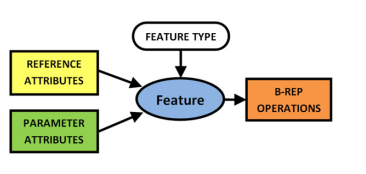
\includegraphics[width=0.5\linewidth]{images/OntologyTessier}
%	\caption{Feature Ontology (Source: \cite{Tessier2013})}
%	\label{fig:litsurvey:Tessier}
%	\end{figure}
	
%\subsection{State of the Art}
%
%\csvreader[longtable=|p{0.15\linewidth}|p{0.1\linewidth}|p{0.1\linewidth}|p{0.25\linewidth}|p{0.15\linewidth}|p{0.15\linewidth}|,
%    table head=\toprule \bfseries Author & \bfseries Input& \bfseries  Method & \bfseries  Approach& \bfseries  Advantages& \bfseries  Limitations \\ \midrule \endhead,% \bottomrule \endfoot,
%  late after last line=\\\bottomrule,
%  before reading={\catcode`\#=12},after reading={\catcode`\#=6},    
%    late after line=\\\hline]%
%{../DocsSources/litsurvey_abstraction.csv}{Author=\Author, Input=\Input, Method=\Method, Approach=\Approach, Advantages=\Advantages ,Limitations=\Limitations}%
%{\Author  & \Input&  \Method &\Approach & \Advantages & \Limitations}%
%
%\subsection{Observations}
%
%%
%\begin{itemize}[noitemsep,topsep=2pt,parsep=2pt,partopsep=2pt]
%	\item In general there has been limited success to the usage of Spatial Grammars in CAD and in the downstream applications, so far, especially for the purpose of neutral {\em feature} definitions.
%	\item  As this work focuses on thin-walled solids, so naturally scopes itself to work on Sheet Metal features. Use of Spatial Grammar notations to represent scheme of generalized {\em form features} is relatively new and is not widely utilized in the commercial CAD applications. 
%\end{itemize}


 
 
\section{Proposed CAD Model Representation}\label{sec:abstraction:proposal}

\added{Objective of this section is to present the generalized feature-based CAD model representation, based on Spatial Grammar. As the existing sheet metal feature based CAD model will be transformed in this new representation, it will need to map all the necessary entities and functionalities of any feature based CAD representation. Requirements for the proposed generalized representation are:}

 \todo{Review Comment: There is no context, rationale as to why you want to propose this (Theoretical background). [CONTEXT AND RATIONALE ADDED. THE WHOLE IDEA IS TO PROPOSE A GENERALIZED CAD MODEL REPRESENTATION AND THEN SHOW HOW MIDSURFACE CAN BE COMPUTED FROM IT. IN THE NEW MODEL REPRESENTATION I EXPLAIN HOW ENTITIES, TRANSFORMATIONS, BOOLEANS AND FEATURES ARE REPRESENTED]}
 
\begin{enumerate}%[noitemsep,topsep=2pt,parsep=2pt,partopsep=2pt]
[noitemsep,topsep=2pt,parsep=2pt,partopsep=2pt]

\item Ability to represent entities needed to build the model, such as line, circle, spline, solid, surface, etc.
\item Ability to specify transformations to spatially place the entities, such as translation, rotation, scaling, etc.
\item Ability to specify a generalized feature that can represent actual features in the model.
\item Ability to specify booleans to join or cut the feature with existing parts.  
\end{enumerate}


 
The sections below present such generalized representation in a terse Spatial Grammar like notation, to transform sheet metal feature CAD model. Midsurface algorithms are then developed based on such generalized feature based CAD model.

The proposed representation is loosely based upon Interactive Configuration Exploration  (ICE) scheme developed by Hoda Moustapha \cite{Hoda2005} for generative designs in architectural domain. Although some of the fundamental entities and syntaxes are borrowed from ICE, the present research enhances it substantially to suit Mechanical CAD application and specifically, for the current context of computation of midsurface.
 
 Following subsections give more details about the ICE scheme, then present how entities, transformations, generalized features and booleans are represented in the proposed approach.
 

 \todo{Review Comment: It is very difficult to comprehend this without any example and its relevance to our problem. Terms, mathematical expressions need to be properly explained with their relevance, context, example and what you want to do with this. [ADDING FIGURE AND EXPLANATION]}
 
 %%-------------------------------------------------------------------------------------------------------------------------------------------------------------------------------------
\subsection{Interactive Configuration Exploration (ICE) Scheme} \label{sec:abstraction:ice}

{\em "The ICE notation is a formalism for describing shapes and  configurations,  by  means  of  their  generative  and  relational  structures"} -- Hoda Moustapha \cite{Hoda2005}.  There are two fundamental entities in ICE, one is a {\em point} shown as $\bar{p}$ and another is called {\em Regulator}, which is an abstraction that represents a unit of action like transformation, constraints, relations, etc. A {\em Regulator} is represented as \\



{\generic{category}{R}{instance}{subtype}{dimension}{arguments}{shapes}}\\

	 For example, Figure \ref{fig:abstraction:hodatranslate} shows the Translation regulator. Its ICE representation is shown below:

	\affine{}{T}{1}{\bar{p},line,n}{shape} 
	
\begin{figure}[!h]
\centering 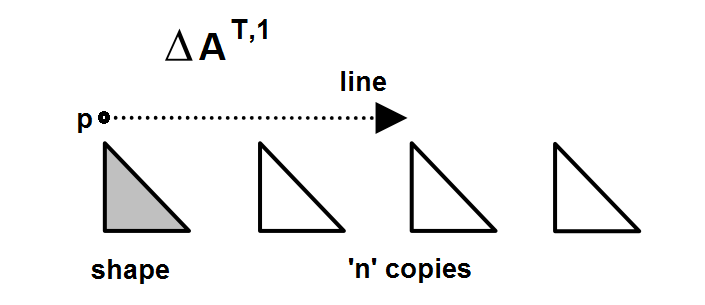
\includegraphics[width=0.5\linewidth]{images/hodatranslate} 
\caption{Translation of a Shape}
\label{fig:abstraction:hodatranslate}
\end{figure}

	
	where,
		\begin{itemize}[noitemsep,topsep=0pt,parsep=0pt,partopsep=0pt]
		\item 	\textcolor{black}{$\Delta$} : Transformation category (type)
	     	\item 	\textcolor{black}{${\bf \mathcal{A}}$} : Affine-transformation regulator (type)
		\item  	\textcolor{black}{$^T$}: subtype Translation (type)
		 \item 	\textcolor{black}{$^1$} : dimensionality of output (integer)
	        \item 	\textcolor{black}{ $\bar{p}$} : position (point)
  		\item  	\textcolor{black}{$line$} : linear guide (curve)
		 \item  	\textcolor{black}{$n$} : number, used for copies, scaling, etc. (float)
		 \item  	\textcolor{black}{$shape$} : target (shape)
		\end{itemize}

%		\begin{itemize}[noitemsep,topsep=0pt,parsep=0pt,partopsep=0pt]
%		\item 	\textcolor{magenta}{$\Delta$} : Transformation category (type)
%	     	\item 	\textcolor{magenta}{${\bf \mathcal{A}}$} : Affine-transformation regulator (type)
%		\item  	\textcolor{magenta}{$^T$}: subtype Translation (type)
%		 \item 	\textcolor{magenta}{$^1$} : dimensionality of output (integer)
%	        \item 	\textcolor{blue}{ $\bar{p}$} : position (point)
%  		\item  	\textcolor{blue}{$line$} : linear guide (curve)
%		 \item  	\textcolor{blue}{$n$} : number, used for copies, scaling, etc. (float)
%		 \item  	\textcolor{red}{$shape$} : target (shape)
%		\end{itemize}
%
The example is of a triangular shape, being translated linearly, from a point $p$, along $line$, with $n$ copies made. It acts as a linear-pattern operation of the triangle.

The ICE notation, can be mapped to Spatial Grammar rules typically represented as $\mathbb{A} \rightarrow \mathbb{B}$. In above example, $(shape)$ is the inputs to the rule, which can be mapped to LHS ($\mathbb{A}$) for the matching condition. On this input, transformation rule $\mathbb{A} \rightarrow \mathbb{B}$ is applied, using specified-arguments in the $\{\bar{p},line,n\}$ to generate RHS ($\mathbb{B}$). More details of the ICE schema are in Appendix \ref{appendix:ice}.
%%Notation is further explained below:
%%
%%\begin{itemize}%[noitemsep,topsep=2pt,parsep=2pt,partopsep=2pt]
%%[noitemsep,topsep=2pt,parsep=2pt,partopsep=2pt]
%%
%%	\item {\em Regulators} are in {\bf bold}, {\bf  $\mathcal{R}$} , represents a unit of action
%%	\item \textcolor{red}{\em shapes} are in {\em lowercase}, say, \textcolor{red}{\em circle, sketch}
%%	\item Prefix to a  {\em Regulator} is its {\em category}, like, \\
%%		 \textcolor{magenta}{$\Delta$}	 :  transformations  \\
%%		 \textcolor{magenta}{$\Phi$} 	 :  constraints  \\
%%		 \textcolor{magenta}{$\Psi$}		 :  hierarchies  \\
%%		 \textcolor{magenta}{$\Pi$}		 :  topologies  \\
%%		 \textcolor{magenta}{$\Xi$}		 : variations  \\
%%		 \textcolor{magenta}{$\Omega$}  :  operations
%%
%%	\item Superscripted$^{suffixes}$  indicate  regulator  {\em subtype},  for instance, \textcolor{magenta}{$\Delta C^p$} and  \textcolor{magenta}{$\Delta C^e$}  respectively specify parabolic and elliptical curve regulators
%%
%%	\item Numerical$^{suffixes}$ denote the dimension of the {\em Regulator}, for instance, \textcolor{magenta}{$\Delta M^0$} ,   \textcolor{magenta}{$\Delta M^1$ }, and   \textcolor{magenta}{$\Delta M^2$}, respectively represent a mirror point (0-dimensions), a mirror line (1-dimension) and a mirror plane (2-dimensions)
%%
%%	\item  Subscripted$_{suffixes}$ for {\em Regulators,  shapes} represent  as  indices;  for  example  \textcolor{magenta}{$\Delta T_1$},  and  \textcolor{magenta}{$\Delta T_2$} are  two different instances of {\em Translation Regulators} used in the same configuration.
%%
%%	\item {\em Regulators} can be generative or non-generative.  Generative  regulators (depicted by the presence of the ``n'' parameter)  take  an  input  shape  and  create output  shapes,  while  non-generative  regulators  act  on  the  input  shape.
%%
%%	\item \textcolor{magenta}{$\Delta {\bf T}$}\textcolor{red}{($\bar{s})^{<0><1><2>}$}  is  a  discrete  application  generating disjoint points, while  \textcolor{magenta}{$\Delta  {\bf T}$}\textcolor{red}{($\bar{s})^{<0,1,2>}$}  is a continuous application generating a line.  
%%
%%	\item Key-points ($ e$ : endpoint,   $m$ : midpoint,   $s$ : start-point) To access key-points (such as the midpoint): \textcolor{red}{$ shape_A \langle m_1 \rangle$}, length by \textcolor{red}{$shape_A \langle l \rangle$}
%%\end{itemize}
%%
%%
%%The present research formalizes an approach to  the neutral form-feature representation and later uses it to develop the midsurface computation algorithm.



%Hoisl \cite{Hoisl2012} mentioned that a limited set of shapes can be generated using {\em Sweep} in a generic manner. A {\em Sweep} is an operation where moving a shape (called {\em generator}) along a trajectory (called {\em guide curve}) creates variety of shapes. {\em Sweep}, by its strict meaning, is limited by use of a single sketch. A more generic operation is {\em Loft}, where multiple sketches are joined together, along a guide curve. 
%It is found that most of the primitives like {\em Box, Cylinder, Cone, Torus, Sphere} and operators like {\em Extrude, Revolve, Sweep, Loft}, in their simplistic form, can be modeled using a {\em Loft} operator.  
%
%Similarly, operators like {\em Translation, Rotation, Scaling} can be modeled using one generic {\em Affine Transformation} operator. {\em Pattern, Mirror} can also be modeled using the same by taking an additional argument as {\em number of copies}.
%
%Another set of operators that can be uniquely represented as a single operator are {\em  Boolean} operators. {\em Union, Difference, Intersection} work on one {\em target body} and multiple {\em tool bodies} with a difference of only  'which cells to retain' logic.
%
%Such set of core operators has lots of advantages like:
%\begin{enumerate}
%\item Operators can be agnostics to the CAD applications. CAD applications may call them differently but the kernel calls could be same.
%\item Data interoperability could be easier as operators are few, neutral and standardized.
%\item Algorithms based on them can be easily ported to different applications, e.g. Midsurface Extraction developed on such core operators can then be ported to in any CAD-CAE application honoring them.
%\end{enumerate}
%
%In many CAD applications, operators are presented as a combination, e.g. {\em  Extrude}, apart from parameters such as {\em sketch} and {\em direction-length}, can ask choice of {\em boolean} and {\em draft-angle}. In the representation scheme presented below, internal {\em booleans} are decoupled from the feature and are modeled separately  i.e. {\em Extrude} will create just the {\em tool body} which will be {\em boolean-ed} later.


%\section{Proposed Feature Generalization Approach  ($\mathcal{ABLE}$) }

%%Objective of proposing a new feature representation scheme is to come up with a specific-to-generic mapping of form features in the context of CAD. The representation scheme proposed here is loosely based upon Interactive Configuration Exploration  (ICE) scheme developed by Moustapha \cite{Hoda2005}, for architectural designs. Although some the fundamental entities and syntax are borrowed from ICE, the rest has been enhanced it to suit the mechanical CAD application, such as this research.


%\subsection{Proposed enhancements}

\todo{Review comment: This is your very significant contribution and difficult in domain. You have to be very careful and cautious to explain these terms for the reader to appreciate the contribution. [MADE SPECIFIC]}

%To cater to this demand, the concept of {\em Regulator} from ICE has been modified to have \textcolor{magenta}{Operator}, \textcolor{blue}{Guide} and \textcolor{red}{Shape}. \textcolor{magenta}{Operator} consists of Type-Subtype and dimensionality of the output. \textcolor{blue}{Guide} typically has the guide-curve info. \textcolor{red}{Shape} is the one on which the operation happens.
\todo{Don't give feel of hand picked addition deletions, rather explain your approach. [REMOVED THE SPECIFICS AND EXPLAINING RATIONAL AT RELEVANT PLACES]}
%%Although entities like {\em point}, {\em line} are present in ICE but entities and features pertinent to Mechanical CAD are not present. Also treatment given to primitives is different in the proposed approach. The additions to ICE are:
%%\begin{itemize}[noitemsep,topsep=2pt,parsep=2pt,partopsep=2pt]
%%\item {\bf Entities} : CAD objects like {\em profile}, {\em sketch} etc.
%%\item {\bf Regulator}: Changed the definition to include $guide$ (directrix) and removed hard coded $\bar{t}, d$
%%\item {\bf Class Hierarchy} : Inheritance {\em derived::parent} relationships between entities. Operations can be defined in terms of the {\em parent} entities so that they are applicable to {\em Derived} classes as well.\\
%%		$derived::base$ : subclass relationship\\
%%		$|$ : logical OR\\
%%		$\&$ : logical AND
%%\item {\bf Form Features} : Definitions of variety of form feature and operations like patterning etc.
%%\end{itemize}
The proposed representation leverages ICE notation, Spatial Grammar rules and a newly proposed feature generalization schema. 
The proposed generalized CAD model representation is called as {\bf $\mathcal{ABLE}$} (Affine-transformation ($\mathcal{A}$),  Boolean ($\mathcal{B}$) and Loft ($\mathcal{L}$), operating on Entities($\mathcal{E}$)).  It is a new paradigm to represent feature based CAD model. It consists of specifications for CAD transformations (called $\mathcal{ABLE}$  transformations -- $A$), CAD Boolean operations (called $\mathcal{ABLE}$ Booleans -- $B$), CAD features (called $\mathcal{ABLE}$ features -- $L$) and CAD entities (called $\mathcal{ABLE}$ entities -- $E$). The CAD model represented in this paradigm is called as $\mathcal{ABLE}$ model. It satisfies the requirements specified in Section \ref{sec:abstraction:proposal}  and also validates the Hypothesis \ref{hyp:Abstraction} (Section \ref{sec:litsurvey:rquestions}) which states that Loft (and equivalent) feature can be used to represent rest of the sheet metal modeling features. 

Following sub-sections elaborate every aspect of $\mathcal{ABLE}$ representation, i.e. Entities, Affine-transformations, Booleans and Loft. Once the representation is established, the next section presents algorithms to convert existing sheet metal features to $\mathcal{ABLE}$ Loft-equivalent features. Finally, midsurface computation of $\mathcal{ABLE}$ Loft equivalent features is elaborated.

\subsection{Proposed Representation of $\mathcal{ABLE}$ Entities ($\mathcal{E}$)}

This section elaborates how various CAD entities are represented in $\mathcal{ABLE}$.

The fundamental geometric primitive in $\mathcal{ABLE}$ is a {\em point}. All the other geometric  entities are directly or indirectly defined in terms of points. 
Basic tenet of $\mathcal{ABLE}$ is that most of the geometric entities and features can be represented by an operation known as Lofting (or Sweeping). In Lofting, 2D profile are lofted along a guide\_curve. It is a very versatile geometric operation. Table ~\ref{tbl:abstraction:entitiesfeaturesusingable} shows how different shapes can be built by lofting different shapes of 2D profiles along with the different shapes of $guide\_curve$s. 

%%\bigskip

\begin{table}[!htb]
\caption{Sweeping Based Entities}
\label{tbl:abstraction:entitiesfeaturesusingable}
\begin{tabular}[h]{@{}p{0.3\linewidth} p{0.18\linewidth} p{0.18\linewidth} p{0.18\linewidth}@{}}
\toprule
%\backslashbox[1mm]{sketch}{guide} & {\bf line} & {\bf arc} & {\bf curve}\\
\qquad \qquad {\bf Guide}  & {\bf line} & {\bf arc} & {\bf curve}\\
\midrule
{\bf 2D Profile Entity} \quad &  &  & \\
\midrule
{\bf point} & line & arc & curve \\\midrule
{\bf line} & plane  & cylinder & ruled \\\midrule
%{\bf arc} & cylinder  & torus  & saddle  \\\midrule
{\bf open profile} & ruled  & circular  &  free form  \\\midrule
{\bf rectangle} & box & rect torus & rect sweep \\\midrule
{\bf circle} & cylinder & torus   & tube \\\midrule
{\bf closed profile} & Extrude & Revolve  & Sweep \\\midrule
%\bottomrule
\end{tabular}
\end{table}

%%\bigskip

	\begin{figure}[!h]
	\centering     %%% not \center
	\subfloat[Line]{\label{fig_linesweep}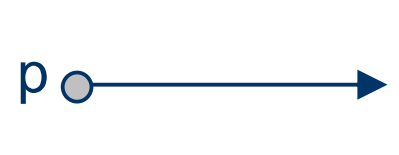
\includegraphics[width=0.28\linewidth]{images/linesweep}}\quad
	\subfloat[Box]{\label{fig_boxsweep}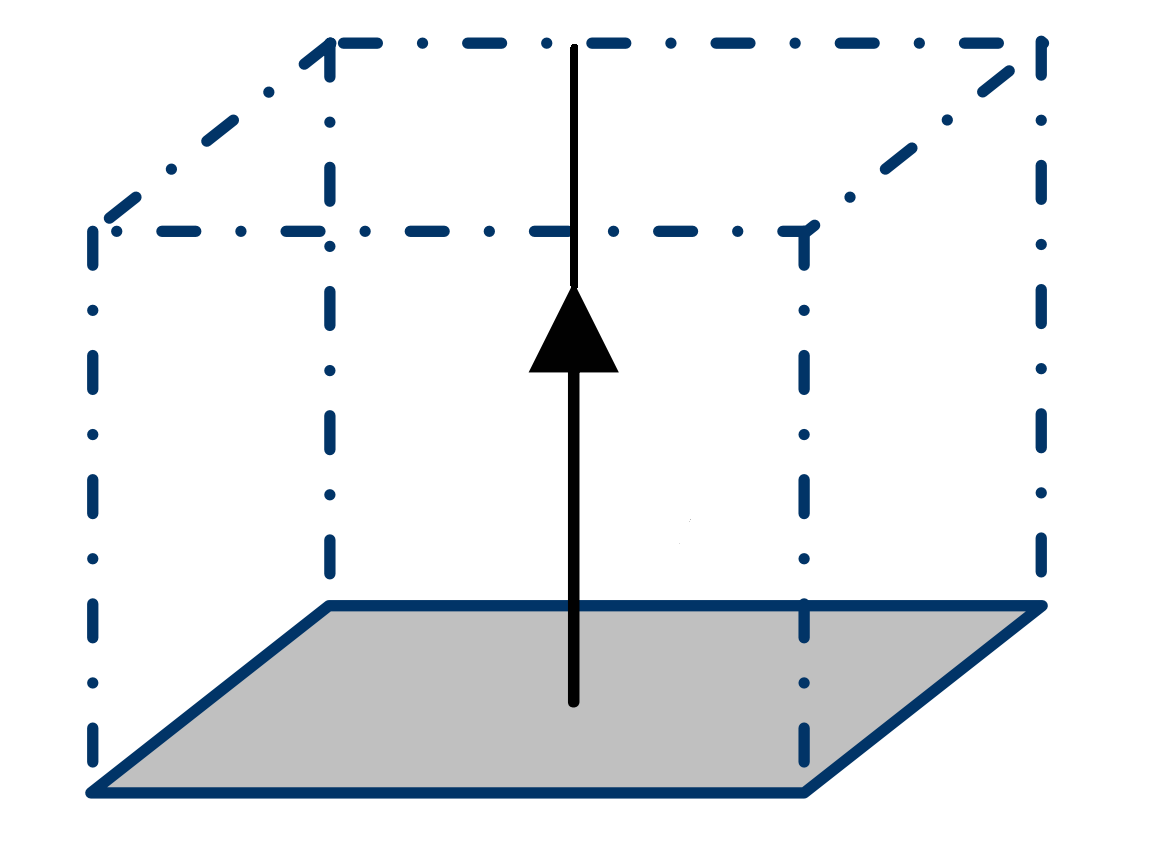
\includegraphics[width=0.28\linewidth]{images/boxsweep}}\quad
	\subfloat[Cylinder]{\label{fig_cylsweep}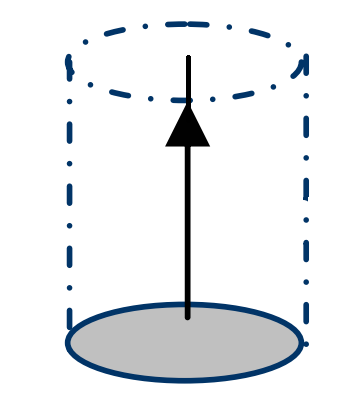
\includegraphics[width=0.2\linewidth]{images/cylindersweep}}
	\caption{Variety of Primitives Created by Sweeping} %%%%%%%% ADD (\{citeYogeshIITG2014}) LATER
	\label{fig_sweptsolids}
	\end{figure}
	
%%\bigskip



For example, Figure~\ref{fig_sweptsolids} shows how Sweeping is used to create basic primitives such as a line, a box and a cylinder. Figure~\ref{fig_linesweep} shows a $point$ as a 2D profile and a $line$ as a $guide$ when swept resulting in a $line$. Figure~\ref{fig_boxsweep} shows a $rectangle$ as a 2D profile and a $line$ as a $guide$ when swept resulting in a $box$.  Figure~\ref{fig_cylsweep} shows a $circle$ as a 2D profile and a $line$ as a $guide$ when swept resulting in a $cylinder$. These results show that Sweep is a versatile operation. Lofting is more generalized than Sweeping operation. Sweeping is done only with one 2D profile and a guide curve, whereas Lofting takes multiple 2D profiles and a guide curve. So, it is not possible to create a cone by sweeping but possible by lofting. Figure~\ref{fig_cone} shows how pyramid and a cone can be modeled using lofting, by giving first 2D profile as $rectangle$ and $circle$ respectively. 

%%\bigskip

\begin{figure}[!h]
\centering 
\subfloat[Pyramid]{\label{fig_pyrloft}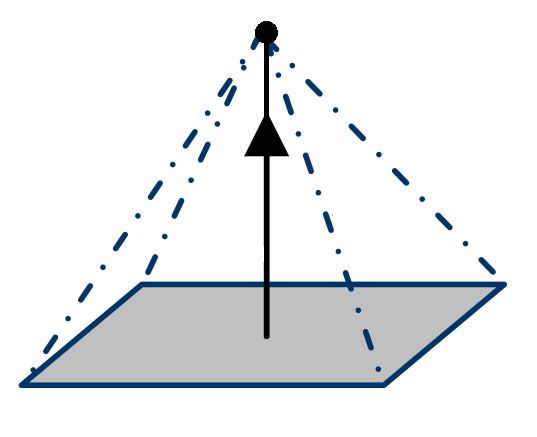
\includegraphics[width=0.25\linewidth]{images/pyrloft}}\quad
\subfloat[Cone]{\label{fig_coneloft}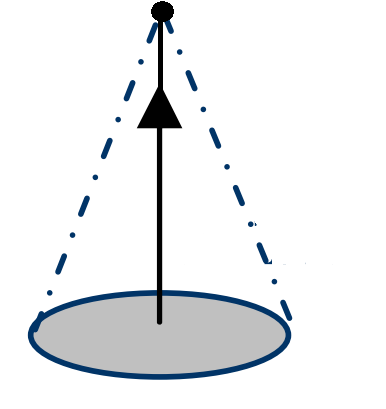
\includegraphics[width=0.25\linewidth]{images/coneloft}}
\caption{Variety of Primitives Created by Lofting}
\label{fig_cone}
\end{figure}

%%\bigskip

Figure~\ref{fig_coneloft} shows, for cone, `2D profile 1' having a circle is lofted to `2D profile 2' having a point, along linear guide curve. Thus Lofting is a very versatile operation and it has been used as a generalized operation for defining entities and features in $\mathcal{ABLE}$.

%%\added{Following entities are useful in defining sketches or guide curves which intern define Loft features. So, the CAD model represented in  $\mathcal{ABLE}$ is defined in terms of geometric entities mentioned below. Such $\mathcal{ABLE}$ model is input to the further steps of computing midsurface. Midsurface is thus indirectly defined as dimension reduction transformation of the $\mathcal{ABLE}$ model. }

\todo{Review comment: A layman question, OK, So? Why should we be concerned. [GAVE EXPLANATION HERE]}

\added{$\mathcal{ABLE}$ introduces Object Oriented class hierarchy of geometric entities and makes $shape$ as the top most base class, from which rest of the entities are derived. Advantage of such hierarchy is that once any operation is defined on the $shape$ it is automatically applicable to all the entities.} 

\begin{figure}[!h]
\centering 
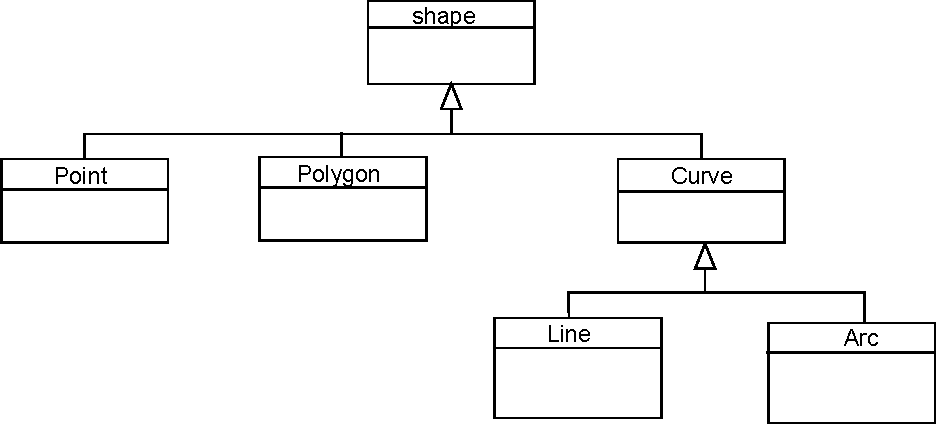
\includegraphics[width=0.8\linewidth]{images/ablehierarchy.pdf} 
\caption{Class Hierarchy of $\mathcal{ABLE}$ Entities}
\label{fig_ablehierarchy}
\end{figure}

Figure~\ref{fig_ablehierarchy} shows the class hierarchy where arrow direction points from derived (child) class to base (parent) class.
Following are some of the relevant entities defined in $\mathcal{ABLE}$:

\begin{itemize}[noitemsep,topsep=2pt,parsep=2pt,partopsep=2pt]

\item {\bf Shape} ($shape$): Topmost base class of Object Oriented class hierarchy for $\mathcal{ABLE}$ entities. All other entities directly or indirectly derive from it. \todo{Review comment: Do you want to explain in Programming language paradigm? I would not recommend. First explain and then present in this form. [EXPLAINED WHAT BASE CLASS MEANS, ABOVE]}


\item {\bf Point} ($point::shape$): It is a fundamental geometric primitive expressed as $\bar{p}$. 	It is derived from base class $shape$.

\item {\bf Line} ($line::curve$): Line is defined by two points and is derived from a generalized class called $curve$. Figure~\ref{fig:abstraction:hodaline} shows a $line$ defined by two points ($\bar{s_1}$ and $\bar{s_2}$). In $\mathcal{ABLE}$, it is expressed as a Loft (operation $\Omega$ of type Loft $\mathcal{L}$) of $\bar{s_1}$ along {\em line} with $\bar{s_1}$ as start point and $\bar{s_2}$ as end point.  \loft{}{T}{1} {s_1,line ,0} {\bar{s_2} )^{<1>} }	

\smallskip

\begin{figure}[!h]
\centering 
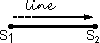
\includegraphics[width=0.2\linewidth]{images/hodaline.pdf} 
\caption{Representation of a Line}
\label{fig:abstraction:hodaline}
\end{figure}

\smallskip


\todo{[IF SUCH DIAGRAMS ARE OK, I WILL GET OTHERS DONE]}

\item  {\bf Arc} ($arc::curve$):  Figure~\ref{fig:abstraction:hodaarc} shows an arc defined by three points, embedding angle $\theta$ and is expressed as a Loft of $\bar{s}_1$ along circular guide with axis $\bar{t}$ and angle $\theta$. \loft{}{R}{1} {s_1,\bar{t}, \theta,0} {\bar{s_2} )^{<1>}}	

\smallskip

\begin{figure}[!h]
\centering 
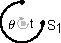
\includegraphics[width=0.12\linewidth]{images/hodaarc.pdf} 
\caption{Representation of an Arc}
\label{fig:abstraction:hodaarc}
\end{figure}

\smallskip


\item {\bf Circle} ($circle::curve$) An $arc$ with full rotation, thus having $\theta = 2\pi$ and is expressed as a Loft of $\bar{s}$ along circular guide with axis $\bar{t}$ and angle $2\pi$ i.e. a full circle. \loft{}{R}{1} {\bar{p},\bar{t}, 2\pi,n} {\bar{s} )^{<0-1>}} 

\item {\bf Curve} ($curve::shape$): It is a generalized curve entity modeled in terms of $n$ points expressed as \loft{}{C}{1} {0,0,C_{0|1|2}} {\bar{s} )^{<1-n>}} . It is a curve passing through $n$ points $\bar{s}$.

\item {\bf Polygon} ($polygon::shape$): It is a collection of connected lines. Figure~\ref{fig:abstraction:hodapolygon} shows a polygon as collection (${\Pi}\mathcal{C}$) of $n$ connected $line$ segments and is expressed as \generic{\Pi}{C}{}{P}{1}{C_0}{line)^{<1-n>}}	

\smallskip

\begin{figure}[!h]
\centering 
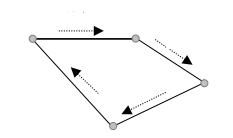
\includegraphics[width=0.35\linewidth]{images/hodapolygon} 
\caption{Representation of a Polygon}
\label{fig:abstraction:hodapolygon}
\end{figure}

\smallskip

\item {\bf Profile} ($profile::shape$): It is a collection of $n$ connected $curve$ segments and  is expressed as \generic{\Pi}{C}{}{P}{1}{0,0,C_{0|1|2}}{curve)^{<1-n>}} 

\item {\bf Sketch} ($sketch::shape$): It is a collection of $profiles$, first outer and rest  inner  and is expressed as \generic{\Pi}{C}{}{S}{1}{}{profile)^{<1><2-n>}}		

\item {\bf Ruled Surface} ($ruledSurface::shape$): It is generated by sweeping of a curve along a line and is expressed as \loft{}{T}{2} {0, curve,0} {line}

Figure~\ref{fig:abstraction:hodasurface} shows a ruled surface modeled using collection of $U,V$ curves and is expressed as \loft{}{F}{2} {0,curve{^{<1-n>} },C_{0|1|2}} {curve{^{<1-m>} }}   

\smallskip

\begin{figure}[!h]
\centering 
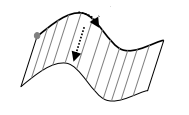
\includegraphics[width=0.35\linewidth]{images/hodasurface} 
\caption{Representation of a Ruled Surface}
\label{fig:abstraction:hodasurface}
\end{figure}

\smallskip

\item {\bf Solid} ($solid::shape$): It is modeled using generic surfaces and is expressed as 

\generic{\Pi}{C}{}{R}{3}{0,0,C_{0|1|2}} {surface{^{<1-n>} }}

\end{itemize}

This subsection presented definitions of some of the $\mathcal{ABLE}$ entities. The next section presents how they can be transformed to position them spatially.

%-----------------------------------------------------------------------------------------------------------------------------------------------------

\subsection{Proposed Representation of $\mathcal{ABLE}$ Affine-transformations ($\mathcal{A}$)}

Affine-transformations use matrix multiplications to translate, rotate, scale entities. Such transformations are needed to place, resize the entities at appropriate location. 

All these are generically clubbed together under {\bf $\mathcal{A}$} with subtypes as $T,R,S$ for {\em Translation}, {\em Rotation} and {\em Scaling} respectively. The value near the sub-type ${0|1|2|3 }$ shows that these actions can be performed on entities of various dimensions, like $point (0)$, $curves(1)$, $surface(2)$ and $solid(3)$. 


\begin{itemize}[noitemsep,topsep=2pt,parsep=2pt,partopsep=2pt]
\item {\bf Translation} moves $shape$, along $line$. Figure~\ref{fig:abstraction:hodatrans} shows translation of a triangular shape.It is expressed as 
\affine{}{T}{0|1|2|3 }{0,line,0} {shape}. 

%\smallskip

\begin{figure}[!h]
\centering 
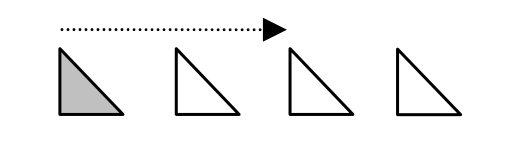
\includegraphics[width=0.35\linewidth]{images/hodatranslationterse} 
\caption{Representation of Translation}
\label{fig:abstraction:hodatrans}
\end{figure}

%\smallskip


\item{\bf Rotation} rotates $shape$, along $arc$ about point $\bar{p}$.  Figure~\ref{fig:abstraction:hodarot} shows rotation of a triangular shape.It is expressed as 	
\affine{}{R}{0|1|2|3 }{0,arc,0} {shape}.
	
%
%\smallskip

\begin{figure}[!h]
\centering 
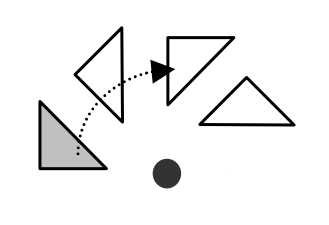
\includegraphics[width=0.35\linewidth]{images/hodarotation} 
\caption{Representation of Rotation}
\label{fig:abstraction:hodarot}
\end{figure}

%\smallskip




\item {\bf Scaling} scales $shape$, by factor  $f$, about $axis$.  Figure~\ref{fig:abstraction:hodascale} shows scaling of a triangular shape. It is expressed as 
\affine{}{S}{0|1|2|3 }{0,axis,f} {shape}.
%\smallskip

\begin{figure}[!h]
\centering 
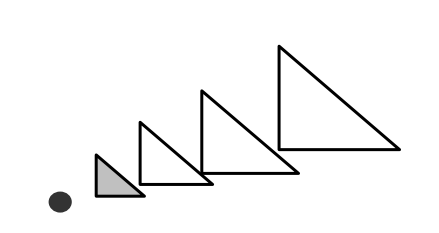
\includegraphics[width=0.35\linewidth]{images/hodascaling} 
\caption{Representation of Scaling}
\label{fig:abstraction:hodascale}
\end{figure}

%\smallskip

\end{itemize}


Copy commands like {\em Pattern} are special cases of {\em Affine-transformations} with an additional parameter of $n$ copies.

\begin{itemize}[noitemsep,topsep=2pt,parsep=2pt,partopsep=2pt]
\item {\bf Linear Pattern} copies $shape$ linearly and is expressed as 

\affine{}{T}{0|1|2|3 }{0,line,n} {shape} 
\item {\bf Circular Pattern} copies $shape$ circularly and is expressed as 

\affine{}{R}{0|1|2|3 }{0,arc,n} {shape} 
\item {\bf Mirror} makes a single copy, mirror-ed about $\bar{t}$. Figure~\ref{fig:abstraction:hodamirror} shows mirroring of a triangular shape. It is expressed as 
\affine{}{M}{0|1|2|3 }{\bar{p},\bar{t}, 0,1} {shape}. 
%\smallskip

\begin{figure}[!h]
\centering 
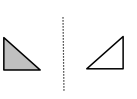
\includegraphics[width=0.35\linewidth]{images/hodamirror} 
\caption{Representation of Mirroring}
\label{fig:abstraction:hodamirror}
\end{figure}

%\smallskip
\end{itemize}

It is often not possible to build described geometries just by positioning pre-defined primitive geometric entities. Complex shapes are built by combines or subtracting from primitive entities. The next section presents boolean operations as defined in  $\mathcal{ABLE}$.
%-------------------------------------------------------------------------------------------------------------------------------------------------------------------------------------

\subsection{Proposed Representation of $\mathcal{ABLE}$ Booleans($\mathcal{B}$)}


Boolean operations are used to unite, difference or intersect two shapes, as denoted by sub-type $U,D,I$ respectively. They are also applicable on dimensionalities like $curve(1)$, $surface(2)$ and $solid(3)$.  Here, first shape, $shape_0$ is regarded as the {\em target body} and the result of the operation is stored in it. Rest of the shapes are termed as {\em tool bodies}.

\begin{itemize}[noitemsep,topsep=2pt,parsep=2pt,partopsep=2pt]
\item {\bf Union} combines all the tool shapes ${shape_{1-k}}$ into master shape, $shape_0$.  Figure~\ref{fig:abstraction:hodaunion} shows union of a box and a ball shape. It is expressed as \boolop{}{U}{1|2|3 }{} {shape_{0-k}}.
%\smallskip

\begin{figure}[!h]
\centering 
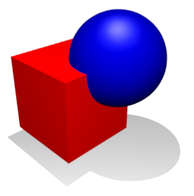
\includegraphics[width=0.35\linewidth]{images/wikiunite} 
\caption{Representation of Union}
\label{fig:abstraction:hodaunion}
\end{figure}

%\smallskip

\item {\bf Difference} removes combination of all the tool shapes ${shape_{1-k}}$ from master shape $shape_0$. Figure~\ref{fig:abstraction:hodasubtract} shows subtraction of a ball from a box shape. It is expressed as \boolop{}{D}{1|2|3 }{} {shape_{0-k}}.

%\smallskip

\begin{figure}[!h]
\centering 
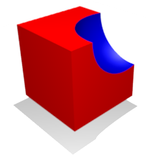
\includegraphics[width=0.3\linewidth]{images/wikisubtract} 
\caption{Representation of Subtraction}
\label{fig:abstraction:hodasubtract}
\end{figure}

%\smallskip





\item {\bf Intersection} keeps only common portion of all the shapes ${shape_{0-k}}$ into master shape $shape_0$. Figure~\ref{fig:abstraction:hodaintersect} shows intersection of a ball and a box shape. It is expressed as \boolop{}{I}{1|2|3 }{} {shape_{0-k}}.	

%\smallskip

\begin{figure}[!h]
\centering 
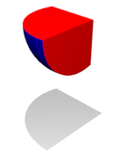
\includegraphics[width=0.23\linewidth]{images/wikiintersect} 
\caption{Representation of Intersection}
\label{fig:abstraction:hodaintersect}
\end{figure}

%\smallskip

\end{itemize}

With entities, transformations and booleans, defined so far it is possible to build CAD model, similar to CSG (Constructive Solid Geometry) representation. As mentioned in Section~\ref{sec:abstraction:proposal}, the present research needs one more set of definitions, i.e. of CAD features. Following section defines generalized representation of $\mathcal{ABLE}$ CAD Features, to be used for converting sheet metal features.

\subsection{Proposed Representation of $\mathcal{ABLE}$ CAD Features}

As mentioned before, the basic tenet of the proposed model is that most of the geometric entities and features can be represented by an operation known as Lofting (or Sweeping). 
The Loft feature is a versatile feature which can represent other CAD features. The present research tests hypothesis \ref{hyp:Abstraction} by demonstrating that sheet metal CAD features model can be represented as Loft feature tree, with suitable transformations and booleans. The transformed generalized CAD model tree is then sent for further steps to compute midsurface.

%%\begin{myhyp} \label{hyp:abstraction:loft}
%%CAD model can be represented as a single or combination of Loft features  having multiple sketches and a guide curve.
%%\end{myhyp}

%In the context of current research, as per Hypothesis \ref{hyp:Abstraction} it is proposed that most of the features can be represented as Loft feature notation and then midsurface transformation is developed on the Loft (and internal Booleans) only.  The input feature tree is converted into Loft tree (Figure \ref{fig:abel}) \cite{YogeshIITG2014}.  This abstracted tree is then sent for Midsurface computation. 


%---------------------------------------------------------------------------------------------------------------------------------------------------------------------------------------------
%\subsubsection{Loft Operators ($\mathcal{L}$)}

Loft is a generic feature capable of generating most of the other features. It joins $sketches$ along a $guide\_curve$.  

\begin{figure}[htbp]
\centering
	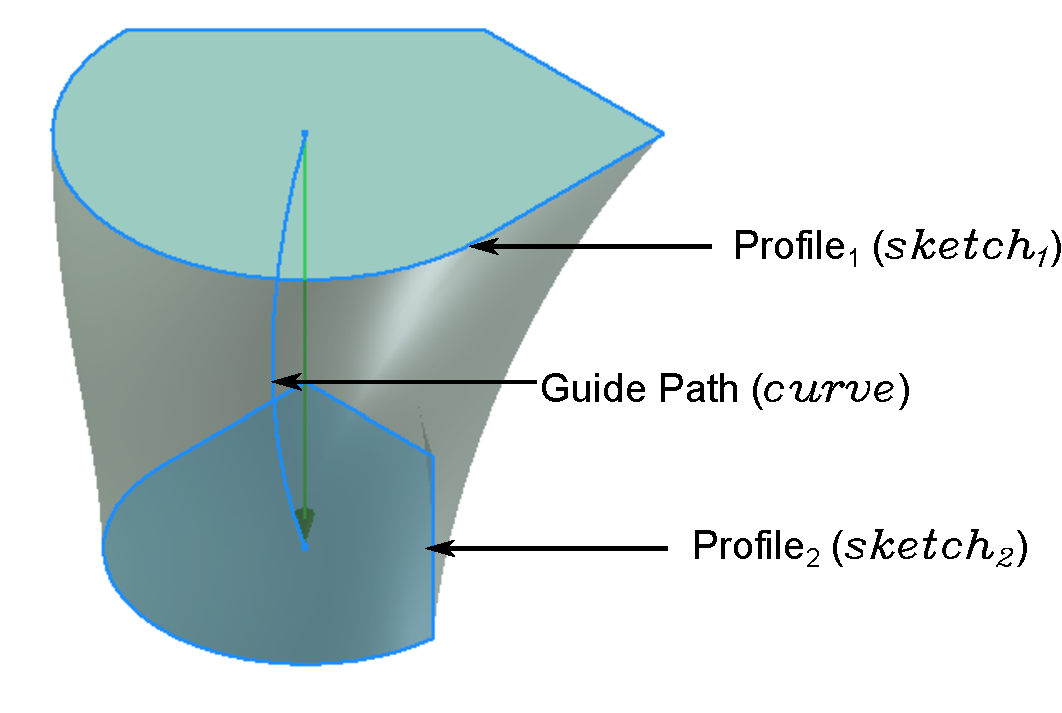
\includegraphics[scale=0.5]{images//LoftPreview.pdf} 
	%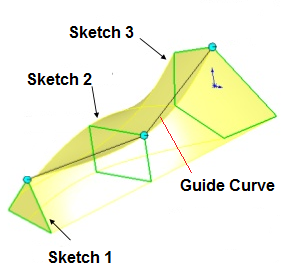
\includegraphics[scale=0.75]{images//LoftPreviewNew1} 
%	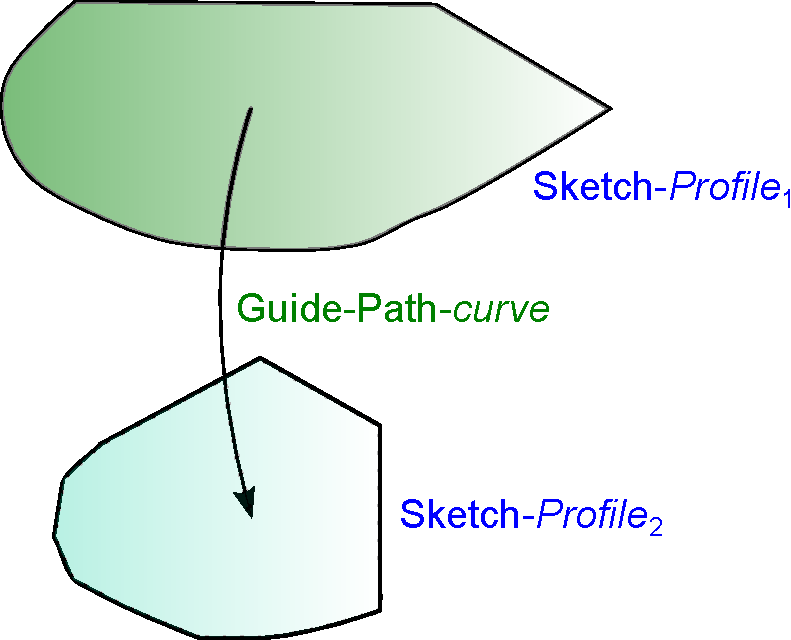
\includegraphics[scale=0.3]{images//LoftProfilesPath.pdf} \\
\caption{Generic Loft Feature}
\label{fig:abstraction:loftschematics}
\end{figure}



Figure \ref{fig:abstraction:loftschematics} shows a Loft having multiple sketches and a guide curve. 

%%\bigskip



%%\bigskip


\todo{Review Comment: Rather provide non-shaded figures. [WIRE-FRAME FIGURES ARE BIT AMBIGUOUS. CHANGED THE FIGURE TO MORE TRANSLUCENT FIGURE]}
In $\mathcal{ABLE}$ generic Loft is represented as:
\vskip 2mm
\loft{}{subtype}{3}{0, guide, 0 | C_{0,1,2}}{ (sketch )^{<1-n>}}
\vskip 2mm

Where,

		\begin{itemize}[noitemsep,topsep=0pt,parsep=0pt,partopsep=0pt]
		\item 	\textcolor{black}{$\Omega$} : Loft category (type)
	     	\item 	\textcolor{black}{${\bf \mathcal{L}}$} : Loft (type)
		\item  	\textcolor{black}{$^{subtype}$}: subtypes like $R$ for Revolve, $E$ for Extrude, etc. (type)
		 \item 	\textcolor{black}{$^3$} : dimensionality of output, $3$ is for solids (integer).  Output of the Loft can either be $solid$ (where capping faces are put to close the shape) or $surface$ (capping faces are not put) and accordingly dimensionality of $2|3$ can be specified.
  		\item  	\textcolor{black}{$guide$} : guide curve, which can be a line, arc or any other curve
		 \item  	\textcolor{black}{$C_{0,1,2}$} : {\em Continuity} options like $C_0$ for connectedness, $C_1$ for tangency and $C_2$ for curvature continuity can be specified at the ends where body generated by the {\em Loft} joins the existing shape. In case this body is disjoint or is the first one in the scene, no {\em continuity}  is specified.
		 \item  	\textcolor{black}{$sketch$} : sketches a Loft profiles (shape). 
		\end{itemize}

%%		\begin{itemize}[noitemsep,topsep=0pt,parsep=0pt,partopsep=0pt]
%%		\item 	\textcolor{magenta}{$\Omega$} : Loft category (type)
%%	     	\item 	\textcolor{magenta}{${\bf \mathcal{L}}$} : Loft (type)
%%		\item  	\textcolor{magenta}{$^subtype$}: subtypes like $R$ Revolve, $E$ for Extrude, etc. (type)
%%		 \item 	\textcolor{magenta}{$^3$} : dimensionality of output, $3$ is for solids (integer).  Output of the Loft can either be $solid$ (where capping faces are put to close the shape) or $surface$ (capping faces are not put) and accordingly dimensionality of $2|3$ can be specified.
%%  		\item  	\textcolor{blue}{$guide$} : guide curve, which can be a line, arc or any other curve
%%		 \item  	\textcolor{blue}{$C_{0,1,2}$} : {\em Continuity} options like $C_0$ for connectedness, $C_1$ for tangency and $C_2$ for curvature continuity can be specified at the ends where body generated by the {\em Loft} joins the existing shape. In case this body is disjoint or is the first one in the scene, no {\em continuity}  is specified.
%%		 \item  	\textcolor{red}{$sketch$} : sketches a Loft profiles (shape). 
%%		\end{itemize}
		

{\bf Loft} can manifest itself in different forms as elaborated below. Figure \ref{fig:abstraction:extruderevolvesweepasloft} shows, by specific shapes of the sketches and the guide curve, it is possible to get features like Extrude, Revolve, and Sweep. These features also come with a variation known as {\em draft}  for tapering sides. This can be modeled as {\em Loft} between two {\em sketches}, where the second {\em sketch} is offset-ed inside-or-outside.

%%\bigskip

\begin{figure}[htbp]
\centering
	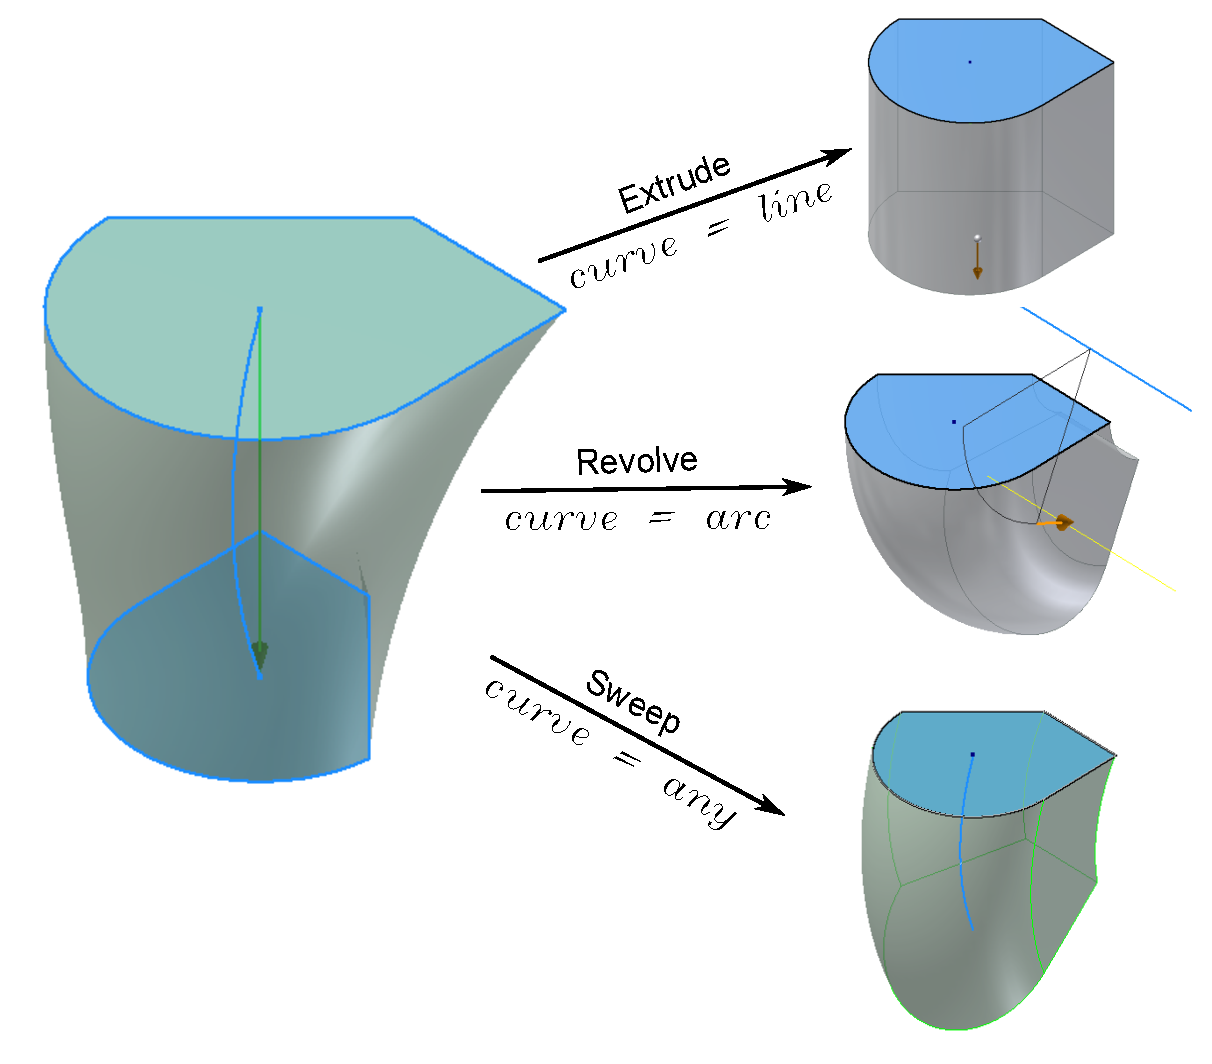
\includegraphics[scale=0.55]{images//LoftExtrudeRevSwp.pdf} 
\caption{Manifestation of Loft Feature into Extrude, Revolve and Sweep}
\label{fig:abstraction:extruderevolvesweepasloft}
\end{figure}

%%\bigskip

\begin{figure}[!h]
\centering 
\subfloat[Extrude without Draft]{\label{fig_extrwodraft}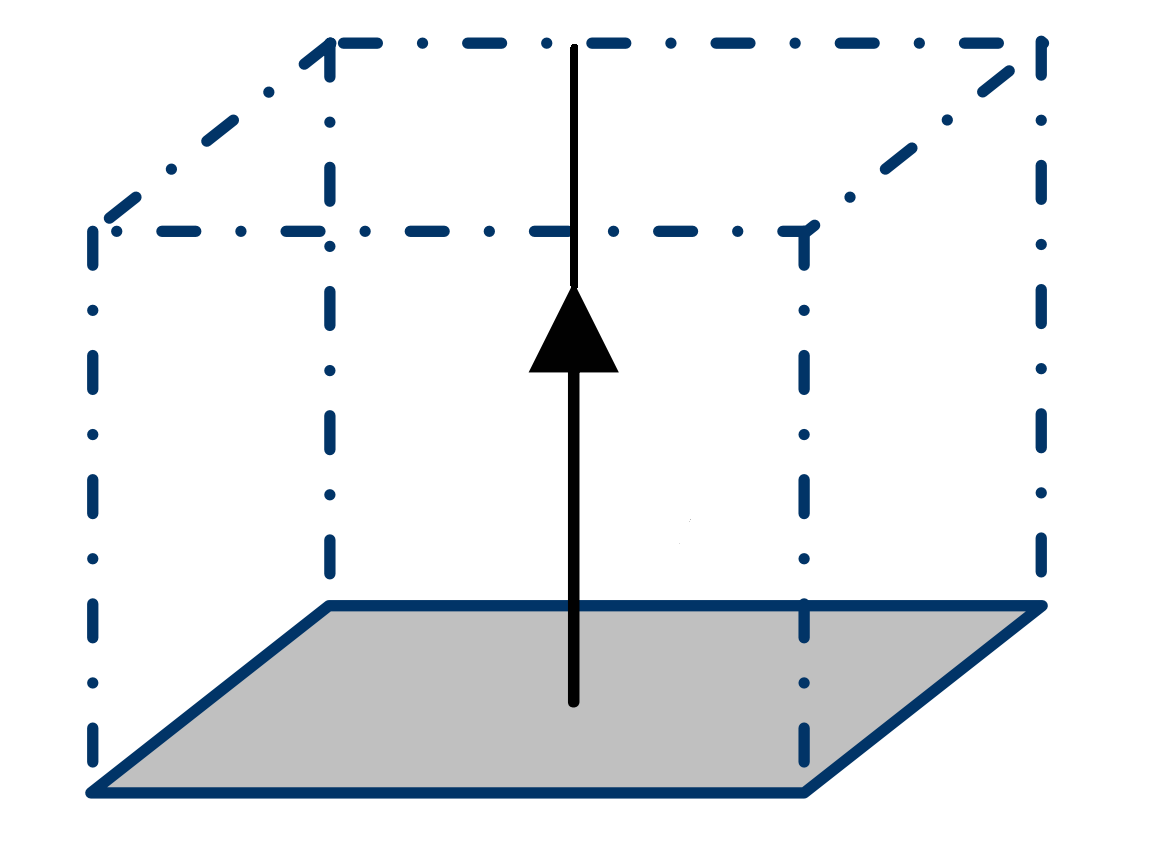
\includegraphics[width=0.3\linewidth]{images/boxsweep}}\quad
\subfloat[Extrude with Draft]{\label{fig_extrudewdraft}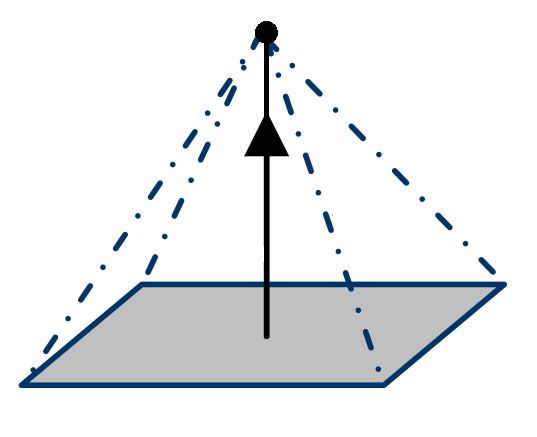
\includegraphics[width=0.3\linewidth]{images/pyrloft}}

\caption{Variants of Extrude}
\label{fig_extrvar}
\end{figure}

%%\bigskip

Each of the features mentioned in Figure~\ref{fig:abstraction:extruderevolvesweepasloft} have two variants, with and without draft. Draft is a tapering operation as explained in Figure~\ref{fig_extrvar}. Figure~\ref{fig_extrwodraft} shows Extrude without any drafting operation, whereas Figure~\ref{fig_extrudewdraft} shows tapering of the side faces, called ``draft''.

\begin{itemize}[noitemsep,topsep=2pt,parsep=2pt,partopsep=2pt]
\item {\bf Extrude}: Extrude without draft is denoted by $EnD$ subtype, has single $sketch$, swept along a $line$ and is expressed as	
\loft{}{EnD}{3 }{0, line, 0 | C_0}{ (sketch )^{<1>}}.
Extrude with draft is denoted by $EwD$ subtype, has two $sketches$ between which loft is made along a $line$ and is expressed as 
\loft{}{EwD}{3 }{0, line, 0 | C_0}{ (sketch )^{<1-2>}}.
\item {\bf Revolve}: Revolve without draft is denoted by $RnD$ subtype, has single $sketch$, swept along an $arc$ and is expressed as
\loft{}{RnD}{3 }{0, arc, 0 | C_0}{ (sketch )^{<1>}}.		
Revolve with draft is denoted by$ RwD$ subtype, has two $sketches$ between which loft is made along an $arc$ and is expressed as
\loft{}{RwD}{3 }{0, arc, 0 | C_0}{ (sketch )^{<1-2>}}.	
\item {\bf Sweep}: Sweep without draft is denoted by $SnD$ subtype, has single $sketch$, swept along a $curve$ and is expressed as	
\loft{}{SnD}{3 }{0, curve, 0 | C_0}{ (sketch )^{<1>}}.		
Sweep with draft is denoted by $SwD$ subtype, has two $sketches$ between which loft is made along a $curve$ and is expressed as
\loft{}{SwD}{3 }{0, curve, 0 | C_0}{ (sketch )^{<1-2>}}.	
\item {\bf Loft} is $n$ sketches between which a loft is made along a generic $curve$ and is expressed as 
\loft{}{L}{3 }{0, curve, 0 | C_{0,1,2}}{ (sketch )^{<1-n>}}. 
\end{itemize}

Primitive shapes are further specializations of {\bf $\mathcal{L}$} operators like {\em Extrude} and {\em Revolve}.  Figure \ref{fig:abstraction:boxcylconeasextrude} shows, by specific shapes of the sketches and the guide curve, it is possible to get primitives such as Box, Cylinder, etc.

%%\bigskip

\begin{figure}[htbp]
\centering
	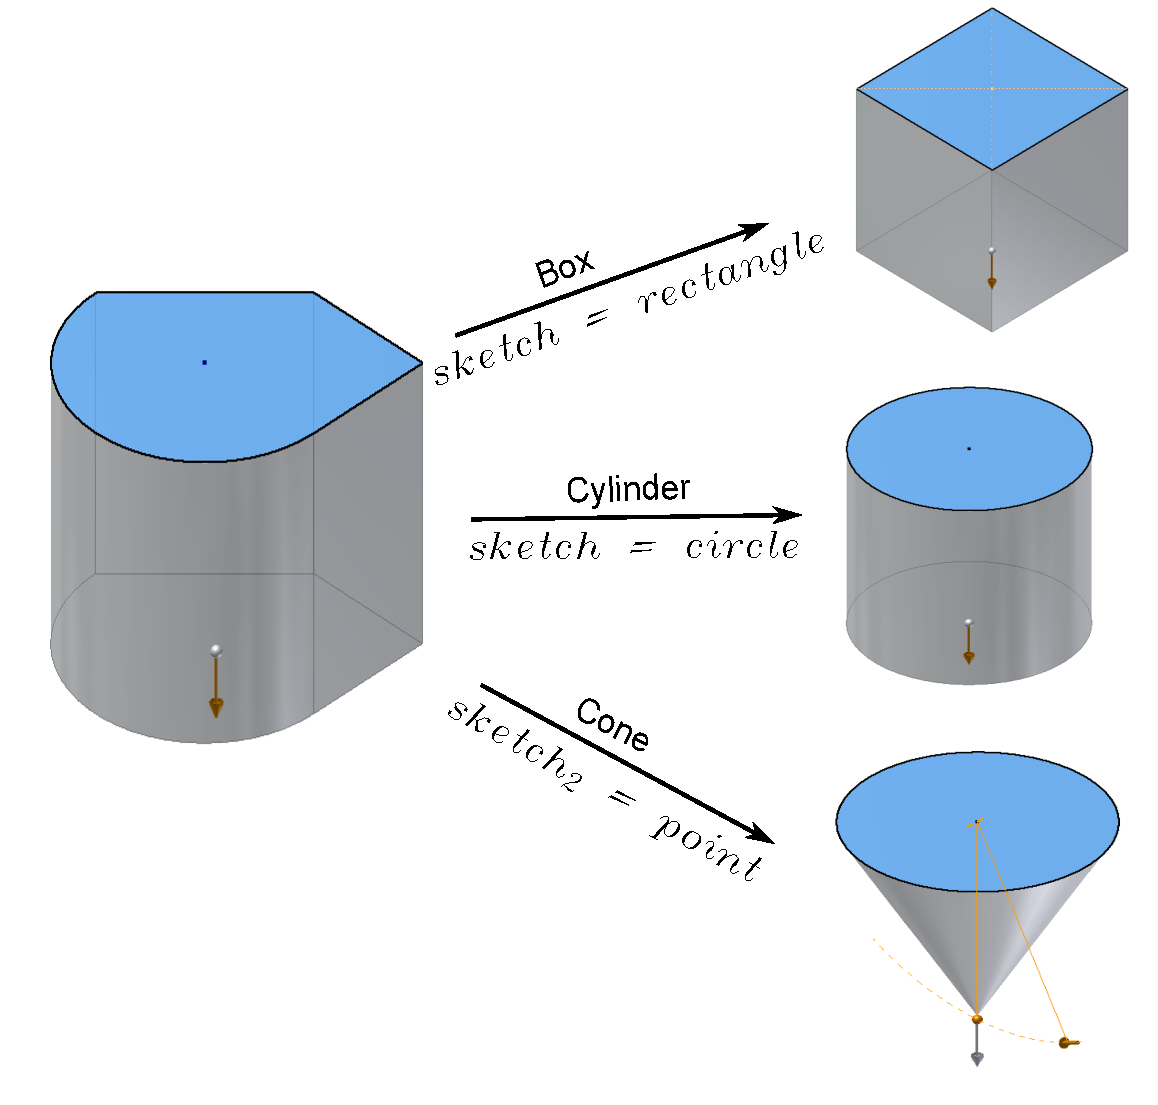
\includegraphics[scale=0.55]{images//ExtrudeBoxCylCone.pdf} 
\caption{Manifestation of  Extrude-Loft feature into Box, Cylinder, Cone}
\label{fig:abstraction:boxcylconeasextrude}
\end{figure}

%%\bigskip

\begin{itemize}[noitemsep,topsep=2pt,parsep=2pt,partopsep=2pt]
\item {\bf Box} : {\em Extrude} with {\em Rectangle} as sketch shape and is expressed as 

\loft{}{EnD}{3 }{0, line, 0 | C_0}{ (rectangle )}	
\item {\bf Cylinder} : {\em Extrude} with {\em Circle} as sketch shape and is expressed as 

\loft{}{EnD}{3 }{0, line, 0 | C_0}{ (circle )}
\item {\bf Cone}: {\em Extrude with draft} with {\em Circle} as first sketch shape, point as second and is expressed as 

\loft{}{EwD}{3 }{0, line, 0 | C_0}{ (circle, point)}
\item {\bf Torus} : {\em Revolve} with {\em Circle} as sketch shape, arc as guide and is expressed as 

\loft{}{RnD}{3 }{0, arc, 0 | C_0}{ (circle)}	
\item {\bf Sphere} : {\em Revolve} with {\em Circle} as sketch shape, point as guide and is expressed as

\loft{}{RnD}{3 }{0, point, 0 | C_0}{ (circle)}	
\end{itemize}

%---------------------------------------------------------------------------------------------------------------------------------------------------------------------------------
%Other features like {\em Shell, Fillet, Chamfer} can be formulated using {\bf $\mathcal{ABLE}$}. 


%Strictly, $\mathcal{L}$oft is a more generic case where the body is created between more than one sketch along the guide curve. Any arbitrary Free From surface is a network of u-v curves and can be imagined as a $\mathcal{L}$oft of multiple $u$ curves along multiple $v$ curves. In the present research, at places, Sweep (which is a single sketch and a single guide curve) is used synonymously for the purpose of clarity.

Following section demonstrates how sheet metal CAD features can be modeled using  $\mathcal{ABLE}$. 

\subsection{Proposed Representation of Sheet Metal Features}\label{sec:abstraction:sheetmetalfeaturesable}
Similar to CAD features, sheet metal features such as Flange, Bend, etc. can also be represented by the generic $\mathcal{ABLE}$ Loft feature as demonstrated in Table~\ref{tbl:abstraction:sheetmetalfeaturesable}. It shows $\mathcal{ABLE}$ representations of sheet metal CAD features.  The first row shows how one of the primary features, called Wall (or ``Face'' in Autodesk Inventor \cite{Inventor2014Help}), is represented in $\mathcal{ABLE}$ as an Extrude 
\loft{}{EnD}{3 }{0, thickness, 0 | C_0}{ (sketch )^{<1>}}. 

It is a Loft $\mathcal{L}$ of sub-type $EnD$, meaning Extrude with no Draft. Its extrusion direction is specified as $thickness$ line. The extrusion profile is denoted by single ($<1>$) $sketch$. The $sketch$ in turn is defined as a collection ($\mathcal{C}$ of sub-type sketch $S$) of one outer profile ($<1>$) and multiple inner profiles ($<2-n>$). The $profile$ is represented as collection  ($\mathcal{C}$ of sub-type profile $P$) of multiple ($<1-n>$) curves. The $curve$ is further defined in terms of multiple points ($\bar{s}$).
 
Next, Bend feature is shown as Sweep \loft{}{SnD}{3 }{0, guide, 0 | C_0}{ (rectangle )^{<1>}}. It is a Loft $\mathcal{L}$ of sub-type $SnD$, meaning Sweep with no Draft. Its sweeping guide curve is specified as $guide$. The sweep profile is denoted by single ($<1>$) $rectangle$. This $rectangle$  is made up of the boundary curves of the thickness face, whose edge is selected for the bending feature. So, the $rectangle$ is defined as a collection ($\mathcal{C}$ of sub-type profile $P$) of4 $lines$. The $guide$ is further defined in terms of multiple points ($\bar{s}$).

Similarly, further examples present $\mathcal{ABLE}$ representations of some of the widely used sheet metal CAD features. As the present research focuses on sheet metal parts and one of the peculiarities of them is that they are of constant thickness. In this case, Sweep, rather than Loft, is the most appropriate generic form for generalization. A sweep is a special case of Loft where, instead of multiple sketches, a single sketch and a guide curve is specified. Extrude and Revolve are special cases of Sweep, so are used interchangeably as Loft-equivalent features.

%%\bigskip

%\begin{table}[!h]
\begin{center}
\captionof{table}{Loft Equivalents ($\mathcal{ABLE}$) of Some Prominent Sheet Metal features}
\label{tbl:abstraction:sheetmetalfeaturesable}
%\resizebox{0.92\linewidth}{!}{ 
\begin{longtable}[htp]{@{}p{0.2\linewidth} | p{0.15\linewidth} | p{0.62\linewidth}@{}}
\toprule
 {\bf Figure } & {\bf Feature} & {\bf $\mathcal{ABLE}$ Features} \\ \midrule

\raisebox{-.9\height}{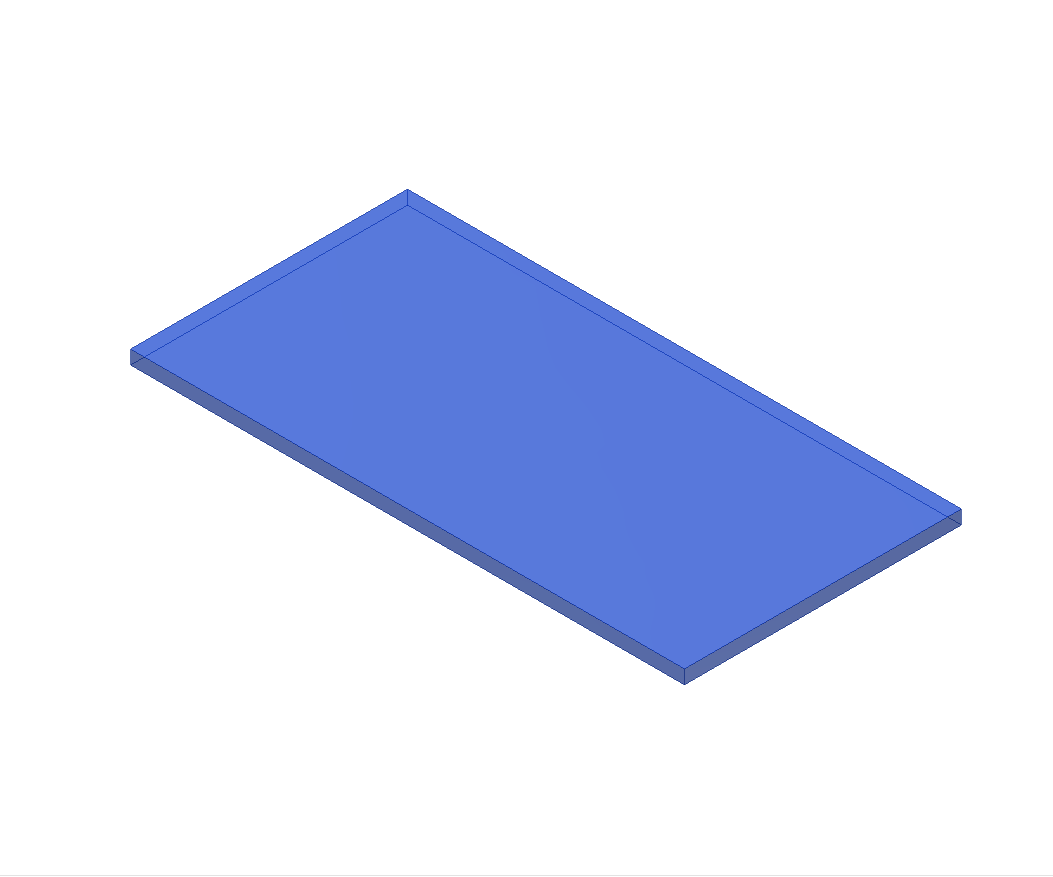
\includegraphics[width=0.98\linewidth]{images/abs_face}} &  {\bf Face, Wall}  & 
{\bf Extrude} is created by extracting $sketch$ of the ``Wall''  feature and giving sheet metal thickness as the distance for extrusion.

\loft{}{EnD}{3 }{0, thickness, 0 | C_0}{ (sketch )^{<1>}}	
Where,

$sketch = $ \generic{\Pi}{C}{}{S}{1}{}{profile)^{<1><2-n>}}

$profile =$ \generic{\Pi}{C}{}{P}{1}{0,0,C_{0|1|2}}{curve)^{<1-n>}}

$curve =$  \loft{}{C}{1} {0,0,C_{0|1|2}} {\bar{s} )^{<1-n>}}
	

\\ \midrule

\raisebox{-.9\height}{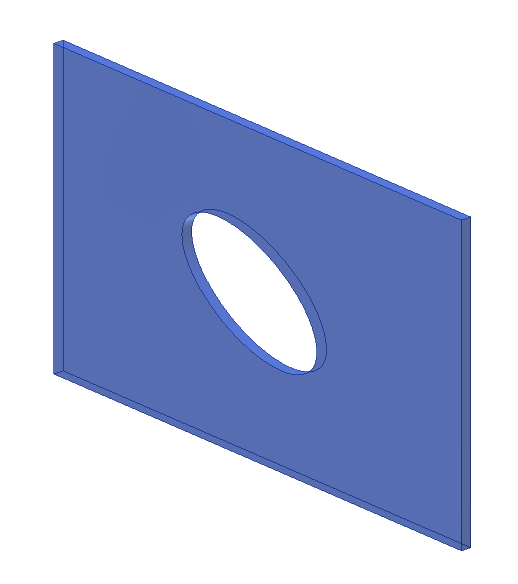
\includegraphics[width=0.8\linewidth]{images/abs_cutout}} &  {\bf Cutout}  & 
{\bf Extrude} is created by extracting $sketch$ of the ``Cutout''  feature and creating hole by ``Subtract'' boolean option.

\loft{}{EnD}{3 }{0, thickness, 0 | C_0}{ (sketch )^{<1>}}	
Where,

$sketch = $ \generic{\Pi}{C}{}{S}{1}{}{profile)^{<1><2-n>}}

$profile =$ \generic{\Pi}{C}{}{P}{1}{0,0,C_{0|1|2}}{curve)^{<1-n>}}

$curve =$  \loft{}{C}{1} {0,0,C_{0|1|2}} {\bar{s} )^{<1-n>}}

And boolean specified as \boolop{}{D}{3}{} {Model, EnD}  

\\ \midrule



  \raisebox{-.9\height}{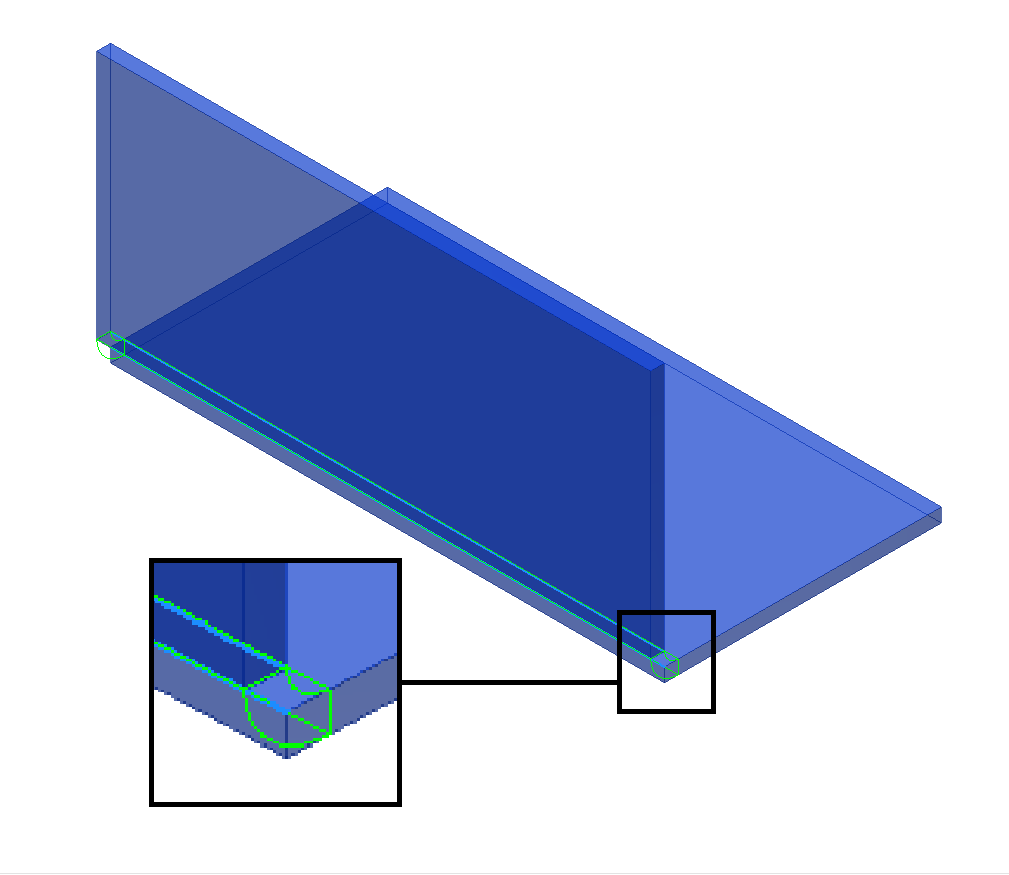
\includegraphics[width=0.98\linewidth]{images/abs_bend_enlarged}} & {\bf Bend}   & 
  {\bf Sweep} is created by creating $guide$ using bend radius and a planar rectangular profile as $sketch$.
    \loft{}{SnD}{3 }{0, guide, 0 | C_0}{ (rectangle )^{<1>}}	
    Where,
    
    $rectangle =$ \generic{\Pi}{C}{}{P}{1}{0,0,C_{0}}{line)^{<1-4>}}
    
    $guide =$  \loft{}{C}{1} {0,0,C_{0|1|2}} {\bar{s} )^{<1-n>}}
    	
%	\begin{algorithmic}
%		\REQUIRE Two Edges
%		\STATE  From first edge, gets it corresponding planar (not rounded) face and create a sketch out of it.
%		\STATE  Using bend radius and starting points of both edges, create guide, then create the sweep
%	\end{algorithmic}
\\ \midrule

 \raisebox{-.9\height}{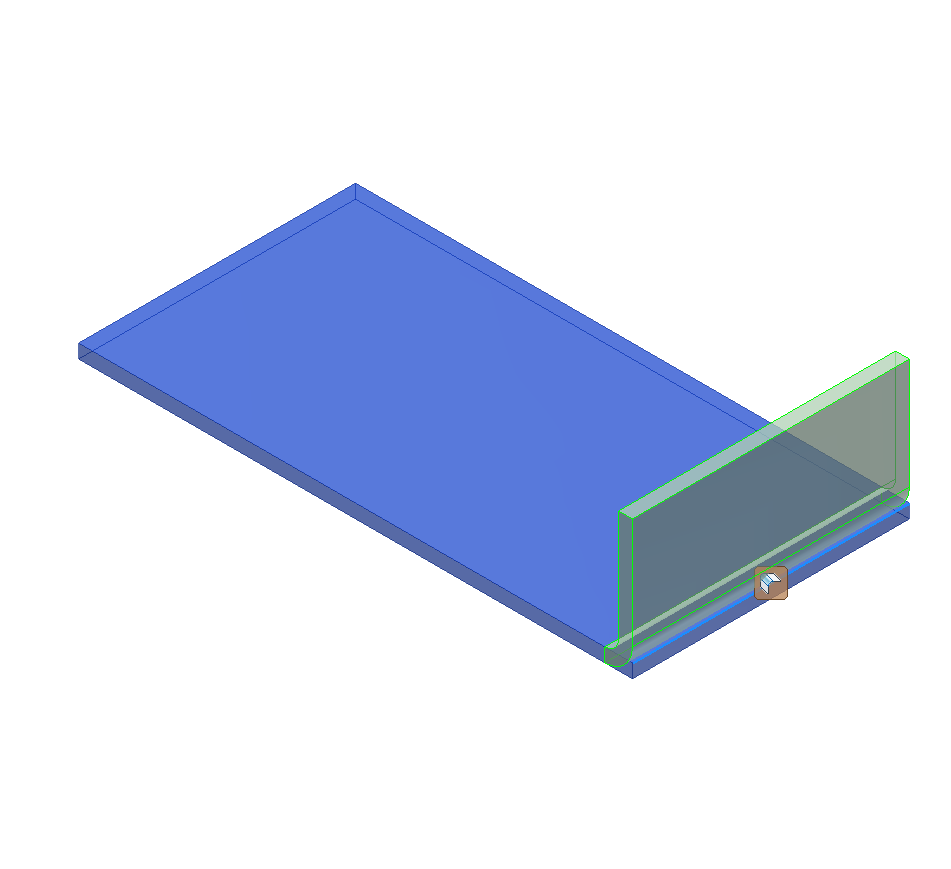
\includegraphics[width=0.98\linewidth]{images/abs_flange}}  & {\bf Flange}   &  
  {\bf Sweep} is created by creating $guide$ using bend radius, offset distance and a planar rectangular profile as $sketch$.
  
  \loft{}{SnD}{3 }{0, guide, 0 | C_0}{ (rectangle )^{<1>}}		
  
%	\begin{algorithmic}
%		\REQUIRE Edge , offset, Bend radius
%		\STATE  Face on which edge was selected is consumed, so we have to rollback before this flange, cache face's geometry as a polyline3d lines, then roll forward.
%		\STATE  The cached geom is then used to create 2 sketches, one for sketch and one for guide
%	\end{algorithmic}
\\ \midrule


 \raisebox{-.9\height}{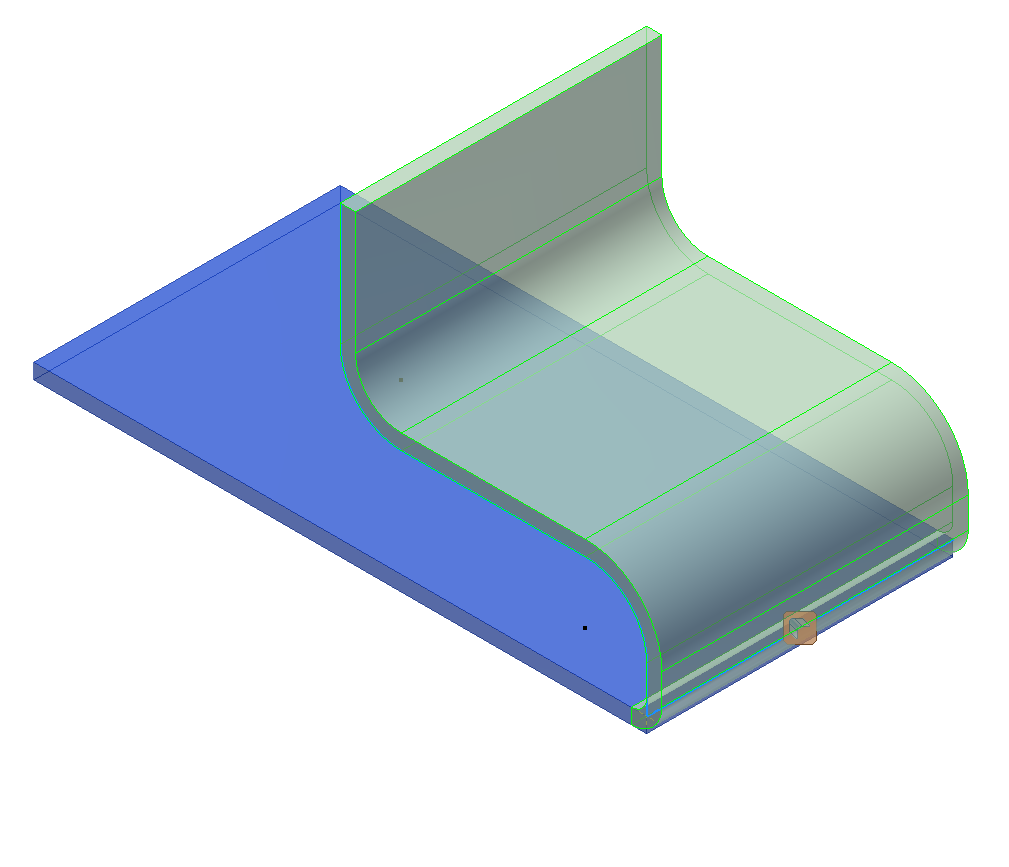
\includegraphics[width=0.98\linewidth]{images/abs_cflange}} &
{\bf Contour Flange }   &  
  {\bf Sweep} is created by creating $guide$ using contour curve and a planar profile as $sketch$.
  
       \loft{}{SnD}{3 }{0, guide, 0 | C_0}{ (rectangle )^{<1>}}		
       
%  	\begin{algorithmic} 
%		\REQUIRE Contour Curve , distance
%		\STATE  While in rollback state, cache curves of contour curve and distance
%		\STATE  Create a new sketch and copy curves in. Offset the curves and add capping lines to make closed sketch
%		\STATE Extrude the sketch
%	\end{algorithmic}
	
%	\begin{algorithmic}
%		\REQUIRE Edge
%		\STATE  While in rollback state,  cache face data similar to FLANGE
%		\STATE  Move the face inside and then prepare contour curve, similar to FLANGE
%		\STATE  SWEEP the sketch along guide
%	\end{algorithmic}
\\ \midrule

 \raisebox{-.9\height}{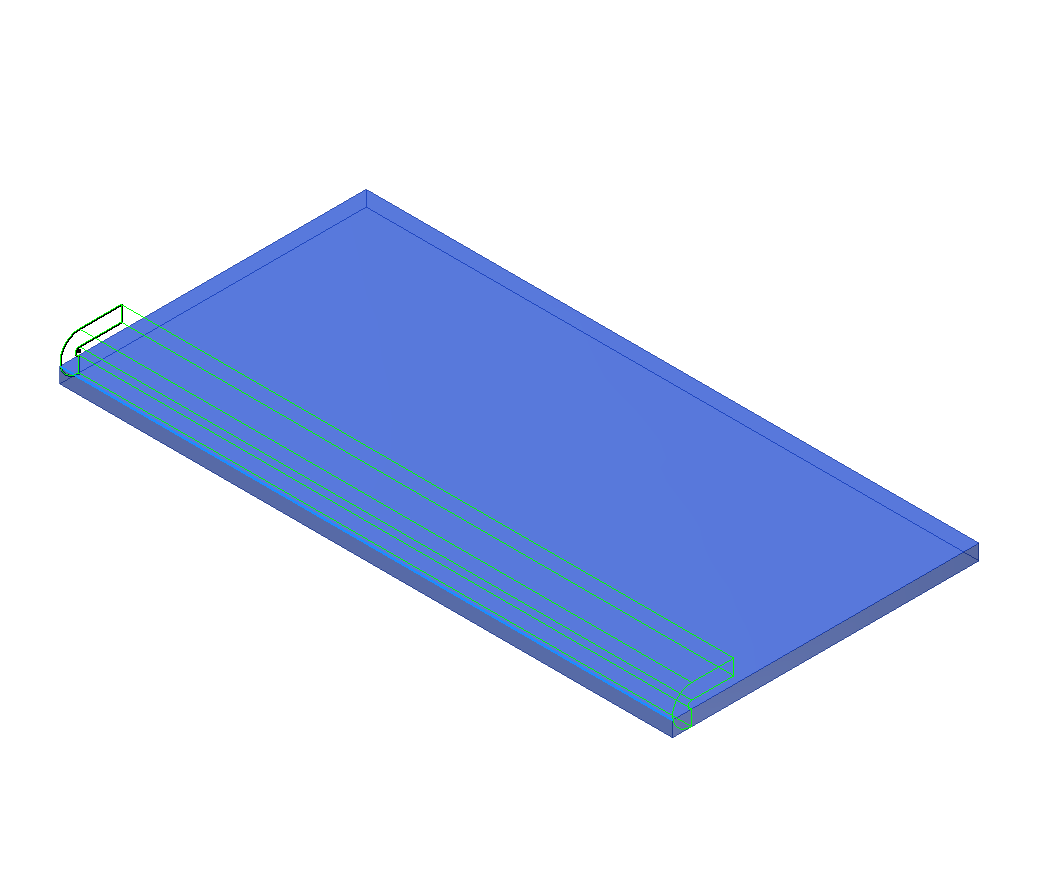
\includegraphics[width=0.98\linewidth]{images/abs_hem}} & 
 {\bf Hem}   &  
   {\bf Sweep} is created by creating $guide$ using hem parameters and a planar rectangular profile as $sketch$.	
   
     \loft{}{SnD}{3 }{0, guide, 0 | C_0}{ (rectangle )^{<1>}}		
     
%	\begin{algorithmic}
%		\REQUIRE Edge , gap, Bend radius
%		\STATE  Face on which edge was selected is consumed, so we have to rollback before this, cache face's geometry as a polyline3d lines, then roll forward
%		\STATE  The cached geom is then used to create 2 sketches, one for sketch and one for guide
%	\end{algorithmic}
\\

\bottomrule
\end{longtable}
%}
\end{center}

%%\bigskip

\todo{Review comment: Add one more column to show inputs in ABLE form i.e. sketches guide etc. [DONE. ADDED SKETCH NOTATION BELOW AS THE SEPARATE COLUMN WOULD NOT BE BIG ENOUGH FOR THE SKETCH EQUATION] }

Apart from sheet metal features, even solid modeling features may be presented as well. They are similarly transformed to their respective Loft-equivalents.
Following section presents algorithms for transforming sheet metal features in the $\mathcal{ABLE}$ representations specified in Table \ref{tbl:abstraction:sheetmetalfeaturesable}.

\section{Transforming Sheet Metal Features CAD Model to $\mathcal{ABLE}$ Model}

\todo{Review comment: This needs to be very detailedly explained wrt each of the  A B L E and conclude with what you have achieved, how your idea is new?. [CHANGED TITTLE FROM `EXAMPLE'. ADDED NEW PARAGRAPH.]}

Previous section explained how entities, affine-transformations, features and booleans are represented in $\mathcal{ABLE}$. This section explains the algorithm for transforming sheet metal CAD model to $\mathcal{ABLE}$ model. It traverses the input model feature tree, and converts each feature one by one to their respective $\mathcal{ABLE}$ features. When an internal or external booleans are encountered, corresponding $\mathcal{AB:E}$ booleans are inserted. Similar transformations and entities are transformed as well. 

\bigskip

\begin{algorithm}[H]
	\caption{Transforming Input CAD Model to $\mathcal{ABLE}$ Model }
	\label{alg:absraction:transform}
	\begin{algorithmic}[1]
		\REQUIRE A Sheet Metal FCAD ($model$) with access to the feature tree
		
%		\WHILE{$nextFace() != null$}
%			\STATE $F_i = currentFace()$
%			\STATE $Area_{face} \quad += F_i \rightarrow area()$
%		\ENDWHILE		
		\WHILE{$model \rightarrow nextFeature() != null$}
			\STATE $f_i = currentFeature()$
			\STATE $af_i \rightarrow converTo\_ABLE\_feature()$
			\STATE $list \rightarrow add(f_i)$
			\STATE $model \rightarrow  add(af_i)$
			\ENDWHILE
		\STATE  $model \rightarrow remove(list)$
		\STATE  $model \rightarrow rebuild()$
	\end{algorithmic}
\end{algorithm}


Algorithm \ref{alg:absraction:transform} presents the overall steps of transformation of input sheet metal features CAD model to $\mathcal{ABLE}$ CAD features i.e. Loft-equivalent features.


%%%\bigskip


%%%\bigskip

\begin{enumerate}
[noitemsep,topsep=2pt,parsep=2pt,partopsep=2pt]
\item The model feature tree is traversed (Algorithm \ref{alg:absraction:transform} lines:1-6 loop). 
\item  The current feature is converted to its Loft-equivalent (Algorithm \ref{alg:absraction:transform} lines: 2-3). 
\item The existing feature is added to a list to be removed later (Algorithm \ref{alg:absraction:transform} line: 4 ). 
\item The converted feature is added to the model (Algorithm \ref{alg:absraction:transform} line: 5). 
\item The features from the old-features-list are removed (Algorithm \ref{alg:absraction:transform} line: 7). 
\item The model is rebuilt (Algorithm \ref{alg:absraction:transform} line: 8).
\end{enumerate}


Following paragraph explains how the function $converTo\_ABLE\_feature()$ (Algorithm \ref{alg:absraction:transform} lines: 3) works for each input CAD feature by taking an example input model shown in Figure \ref{tbl:abstraction:input} and transforming it to $\mathcal{ABLE}$ model as shown in Figure \ref{tbl:abstraction:output}.

\begin{enumerate}
[noitemsep,topsep=2pt,parsep=2pt,partopsep=2pt]
\item The model feature tree which has 5 features,  is traversed  one feature at a time (Algorithm \ref{alg:absraction:transform} lines:1-6 loop). 

\begin{minipage}[t]{0.9\linewidth}
\begin{tabular}[h]{@{} p{0.45\linewidth} | p{0.45\linewidth}@{}} \toprule

\textbf{Input CAD Model} & \textbf{Tree}\\ \midrule

\raisebox{-.9\height}{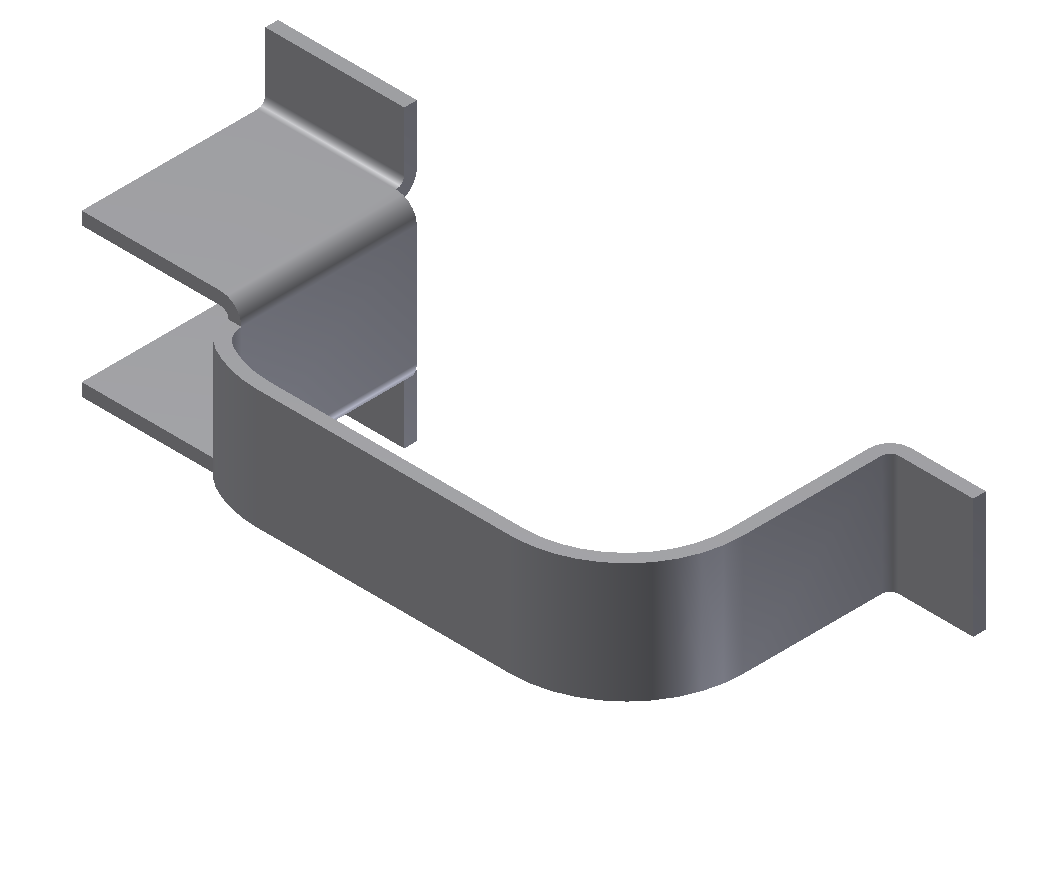
\includegraphics[width=0.98\linewidth]{images/ABELBracketInputPart}}&
\raisebox{-.9\height}{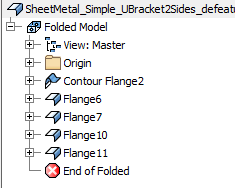
\includegraphics[width=0.98\linewidth]{images/ABELBracketInputTree}} \\ \bottomrule

\end{tabular}
\captionof{figure}{CAD Model Built with Sheet Metal Features}\label{tbl:abstraction:input}
\end{minipage}


\item The first feature encountered is ``Contour Flange2''.  Its parameters are Edge and Contour Curve. Its conversion can be done in one of the two ways, as follows:
	\begin{enumerate}
	[noitemsep,topsep=2pt,parsep=2pt,partopsep=2pt]
	\item Extrude \loft{}{EnD}{3 }{0, distance, 0 | C_0}{ (sketch )^{<1>}} is computed as follows:	
	
	\bigskip
	
			  \begin{minipage}{\linewidth}
		  \begin{algorithm}[H]
			\caption{Contour Flange to $\mathcal{ABLE}$ Extrude}
			\label{alg:absraction:transformextrude}
			\begin{algorithmic}[1]
					\REQUIRE Contour Curve, Edge
					\STATE  While in rollback state, extract Contour Curve from the feature and find length of the Edge and distance.
					\STATE  Sketch creation method 1:  Offset the curves and add capping lines to make closed sketch. Create a new sketch and copy curves in.
					\STATE  Sketch creation method 2:  Extract boundary curves of the face having Contour Curve. Create a new sketch and copy curves in.			
					\STATE Extrude the sketch with the distance.
				\end{algorithmic}
		  \end{algorithm}
		  \end{minipage}	
		  
  \bigskip
  
		Figure~\ref{fig_cf2ext2} shows input feature parameters of Contour Flange and its transformation to equivalent Extrude feature. Algorithm~\ref{alg:absraction:transformextrude} details to steps.
		

		  \begin{minipage}{\linewidth}
		  \begin{figure}[H]
		\centering 
		\subfloat[Contour Flange  Parameters]{\label{fig_cf2}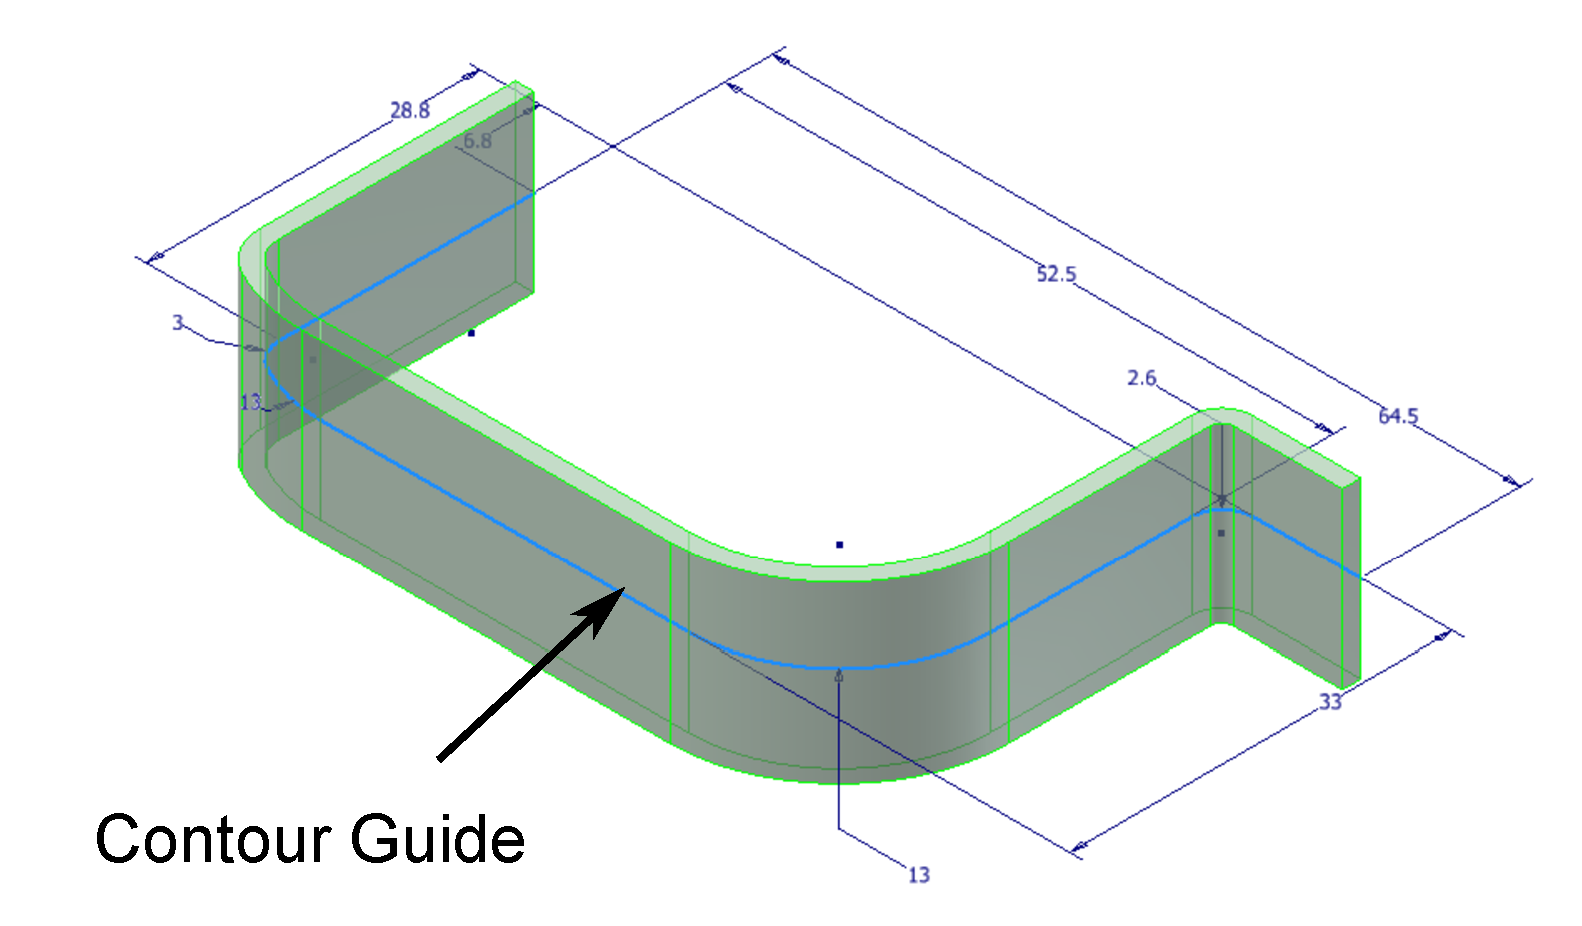
\includegraphics[width=0.48\linewidth]{images/abs_counterflange2edit.pdf}} %\quad
		\subfloat[Extrusion' Parameters]{\label{fig_ext2}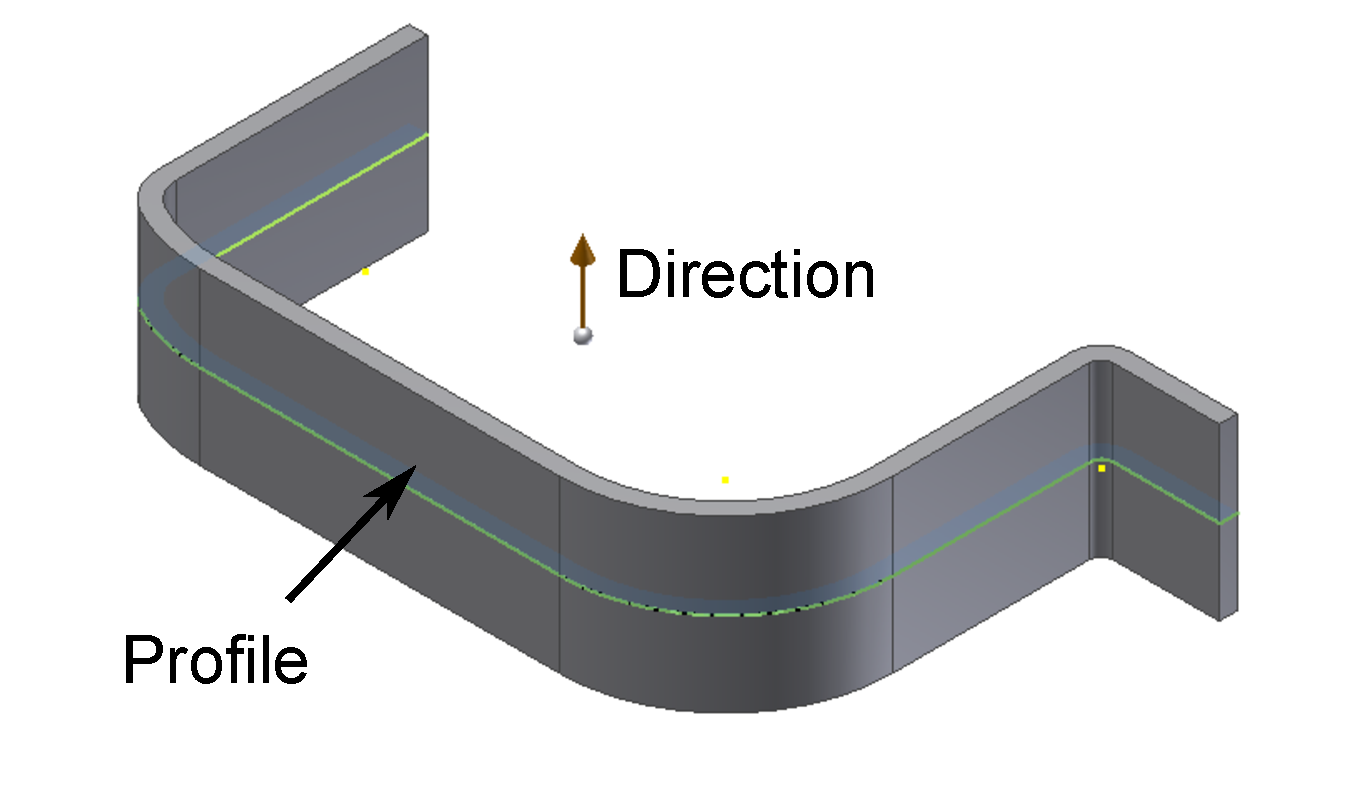
\includegraphics[width=0.4\linewidth]{images/abs_extrude2edit.pdf}}
		\caption{Contour Flange to Extrusion}
		\label{fig_cf2ext2}
		\end{figure}
		\end{minipage}	


%%\bigskip

		  
%%\bigskip			
			
	\item	Sweep   \loft{}{SnD}{3 }{0, guide, 0 | C_0}{ (rectangle )^{<1>}} is computed as follows:	
		
\bigskip
		  \begin{minipage}{\linewidth}
		  \begin{algorithm}[H]
			\caption{Contour Flange to $\mathcal{ABLE}$ Sweep}
			\label{alg:absraction:transformsweep}
			\begin{algorithmic}[1]
					\REQUIRE Contour Curve, Edge
					\STATE  While in rollback state, extract rectangle from thickness Face adjacent to the Edge and the Contour Curve.
					\STATE  Sketch creation method:  Extract boundary curves of the face. Create a new sketch and copy curves in.			
					\STATE  SWEEP the sketch along guide
				\end{algorithmic}
		\end{algorithm}	
		  \end{minipage}				
\bigskip	
	     
	\item Boolean: As this is the first feature, Boolean is not specified.
	\item Output  $\mathcal{ABLE}$ model built so far is:
		\begin{itemize}[noitemsep,topsep=2pt,parsep=2pt,partopsep=2pt,label={+}]
		\item  $Extrusion2 =$ \loft{}{EnD}{3 }{0, edge1, 0 | C_0}{ (sketch1 )^{<1>}}
		\end{itemize}
	\end{enumerate}

\item The second feature encountered is ``Flange6''.  Its parameters are Edge, Flange Distance and Offset distance. Its conversion can be done as follows:
	\begin{enumerate}
	[noitemsep,topsep=2pt,parsep=2pt,partopsep=2pt]
	\item	Sweep   \loft{}{SnD}{3 }{0, guide, 0 | C_0}{ (rectangle )^{<1>}} is computed as follows:	
		
	
	
%%\bigskip


\begin{figure}[!h]
\centering 
\subfloat[Flange Parameters]{\label{fig_fl6}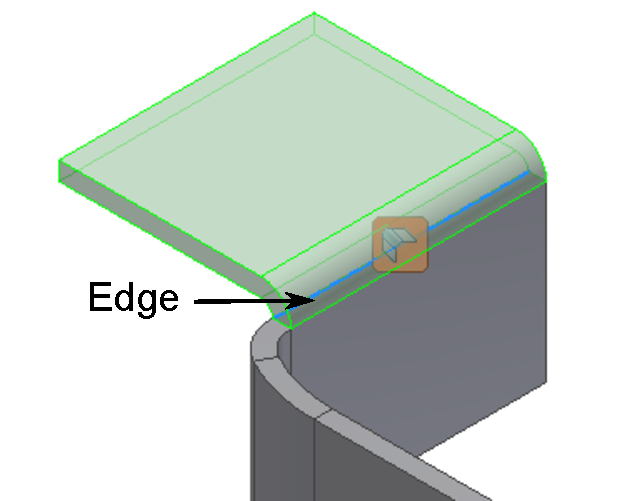
\includegraphics[width=0.32\linewidth]{images/abs_flange6edit.pdf}}\quad
\subfloat[Sweep Parameters]{\label{fig_sw1}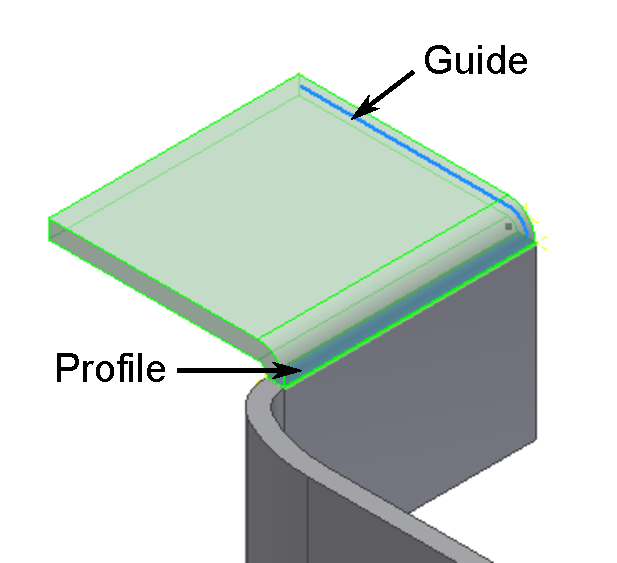
\includegraphics[width=0.32\linewidth]{images/abs_sweep1edit.pdf}}
\caption{Flange to Sweep}
\label{fig_fl6sw1}
\end{figure}

%%\bigskip


Figure~\ref{fig_fl6sw1} shows input feature parameters of Flange and its transformation to equivalent Sweep feature. Algorithm~\ref{alg:absraction:transformsweepflange} details to steps.
		
\bigskip
		  \begin{minipage}{\linewidth}
		  \begin{algorithm}[H]
			\caption{Flange to $\mathcal{ABLE}$ Sweep}
			\label{alg:absraction:transformsweepflange}
			\begin{algorithmic}[1]
					\REQUIRE Edge,  Flange Distance and Offset distance
					\STATE  While in rollback state, extract rectangle from thickness Face adjacent to the Edge.
					\STATE  Sketch creation method:  Extract boundary curves of the face. Create a new sketch and copy curves in.		
					\STATE Guide creation method: Compute 3 connected curves using Offset Distance, Bend Radius and Flange Distance.	
					\STATE  SWEEP the sketch along guide
				\end{algorithmic}
		\end{algorithm}	
		  \end{minipage}				
\bigskip	
	     
	\item Boolean: $Union$ between the second feature with the existing first feature (shown as $model$ so far) and is denoted as: 
	\boolop{}{U}{3}{} {Extrusion2, Sweep1} 	
	\item Output  $\mathcal{ABLE}$ model built so far is:
	
		\begin{itemize}[noitemsep,topsep=2pt,parsep=2pt,partopsep=2pt,label={+}]
		\item  $Extrusion2 =$ \loft{}{EnD}{3 }{0, edge1, 0 | C_0}{ (sketch1 )^{<1>}}
		\item  $Sweep1 =$  \loft{}{SnD}{3 }{0, guide, 0 | C_0}{ (rectangle )^{<1>}},
		
			\boolop{}{U}{3}{} {model, Sweep1} 
		\end{itemize}	
	\end{enumerate}

\item 	Similar transformation happens for the remaining features and the Output  $\mathcal{ABLE}$ model built looks like (Figure \ref{tbl:abstraction:output}), and is shown as follows:
		\begin{itemize}[noitemsep,topsep=2pt,parsep=2pt,partopsep=2pt,label={+}]
		\item  $Extrusion2 =$ \loft{}{EnD}{3 }{0, edge1, 0 | C_0}{ (sketch1 )^{<1>}}
		\item  $Sweep1 =$  \loft{}{SnD}{3 }{0, guide1, 0 | C_0}{ (sketch2 )^{<1>}},
		
			\boolop{}{U}{3}{} {model, Sweep1} 
		\item  $Sweep2 =$  \loft{}{SnD}{3 }{0, guide2, 0 | C_0}{ (sketch3 )^{<1>}},
		
			\boolop{}{U}{3}{} {model, Sweep2} 	
		\item  $Sweep3 =$  \loft{}{SnD}{3 }{0, guide3, 0 | C_0}{ (sketch4 )^{<1>}},
		
			\boolop{}{U}{3}{} {model, Sweep3} 
		\item  $Sweep4 =$  \loft{}{SnD}{3 }{0, guide4, 0 | C_0}{ (sketch5 )^{<1>}},
		
			\boolop{}{U}{3}{} {model, Sweep4} 					
		\end{itemize}	
\end{enumerate}

\bigskip

\begin{minipage}[t]{0.9\linewidth}
\begin{tabular}[h]{@{} p{0.45\linewidth} | p{0.45\linewidth}@{}} \toprule

\textbf{Output $\mathcal{ABLE}$ based Model} & \textbf{Tree}\\ \midrule

\raisebox{-.9\height}{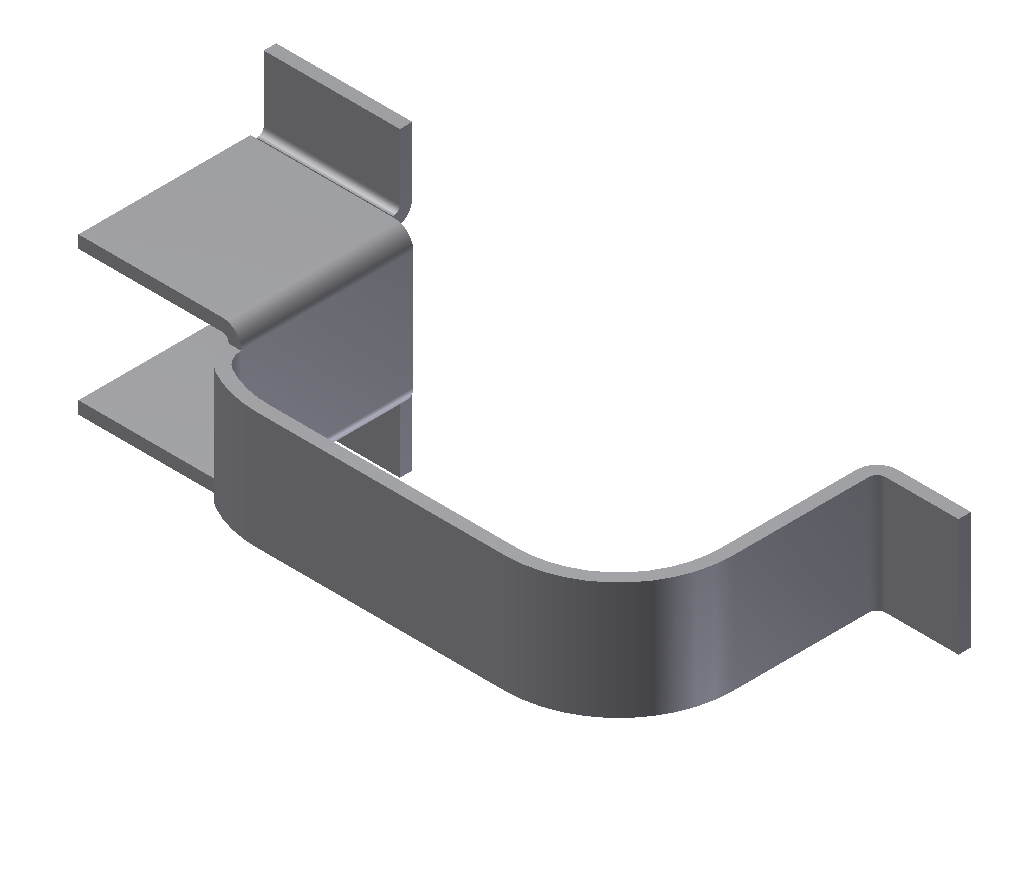
\includegraphics[width=0.98\linewidth]{images/ABELBracketOutputPart}}&
\raisebox{-.9\height}{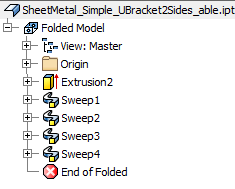
\includegraphics[width=0.98\linewidth]{images/ABELBracketOutputTree}} \\ \bottomrule

\end{tabular}
\captionof{figure}{Output $\mathcal{ABLE}$ Based Model}\label{tbl:abstraction:output}
\end{minipage}

%%\bigskip


%Figure \ref{fig:abel} shows that the model remains the same only the features change. 
%
%%%\bigskip
%
% 
%\begin{minipage}[t]{0.9\linewidth}
%\begin{tabular}[h]{@{} p{0.24\linewidth} p{0.2\linewidth} |  p{0.24\linewidth}  p{0.2\linewidth}@{}} \toprule
%
%\textbf{CAD} & \textbf{Model} & \textbf{$\mathcal{ABLE}$ } & \textbf{Model}\\ \midrule
%
%
%\raisebox{-.9\height}{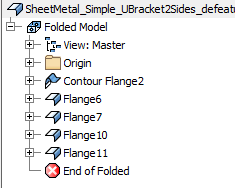
\includegraphics[width=0.98\linewidth]{images/ABELBracketInputTree}}&
%\raisebox{-.9\height}{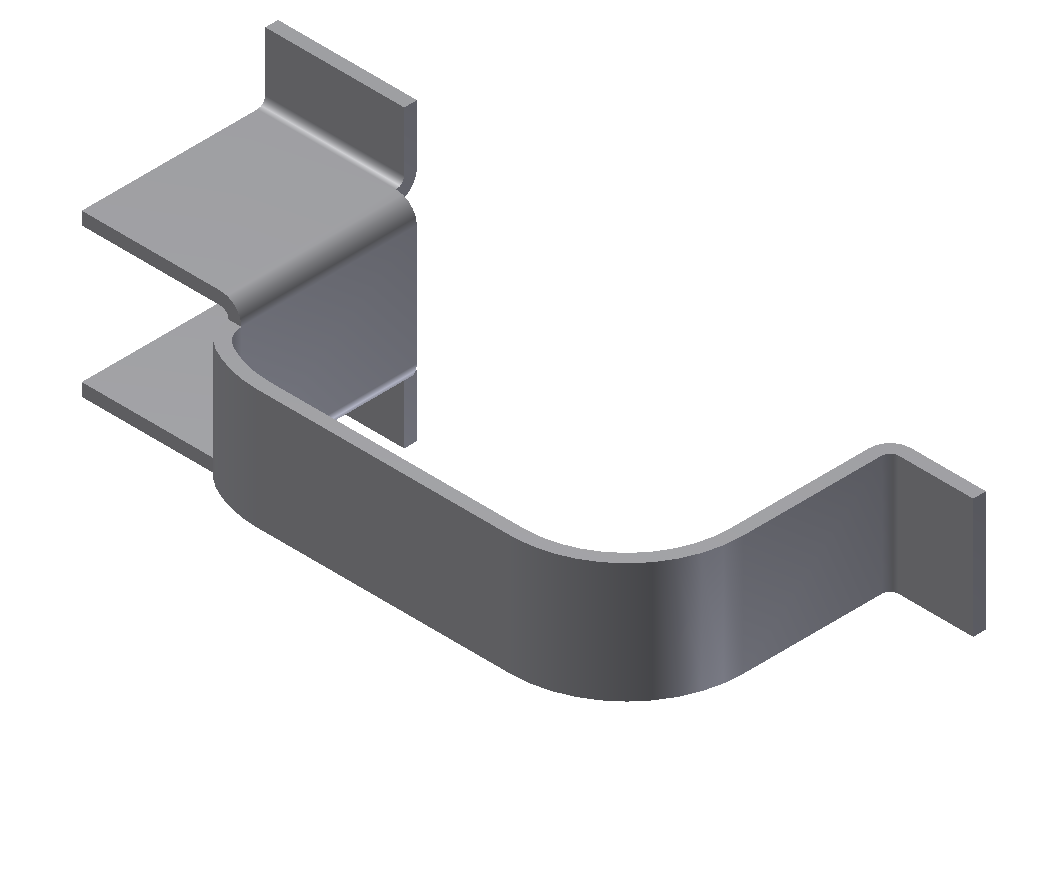
\includegraphics[width=0.98\linewidth]{images/ABELBracketInputPart}} &
%\raisebox{-.9\height}{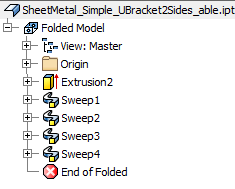
\includegraphics[width=0.98\linewidth]{images/ABELBracketOutputTree}} &
%\raisebox{-.9\height}{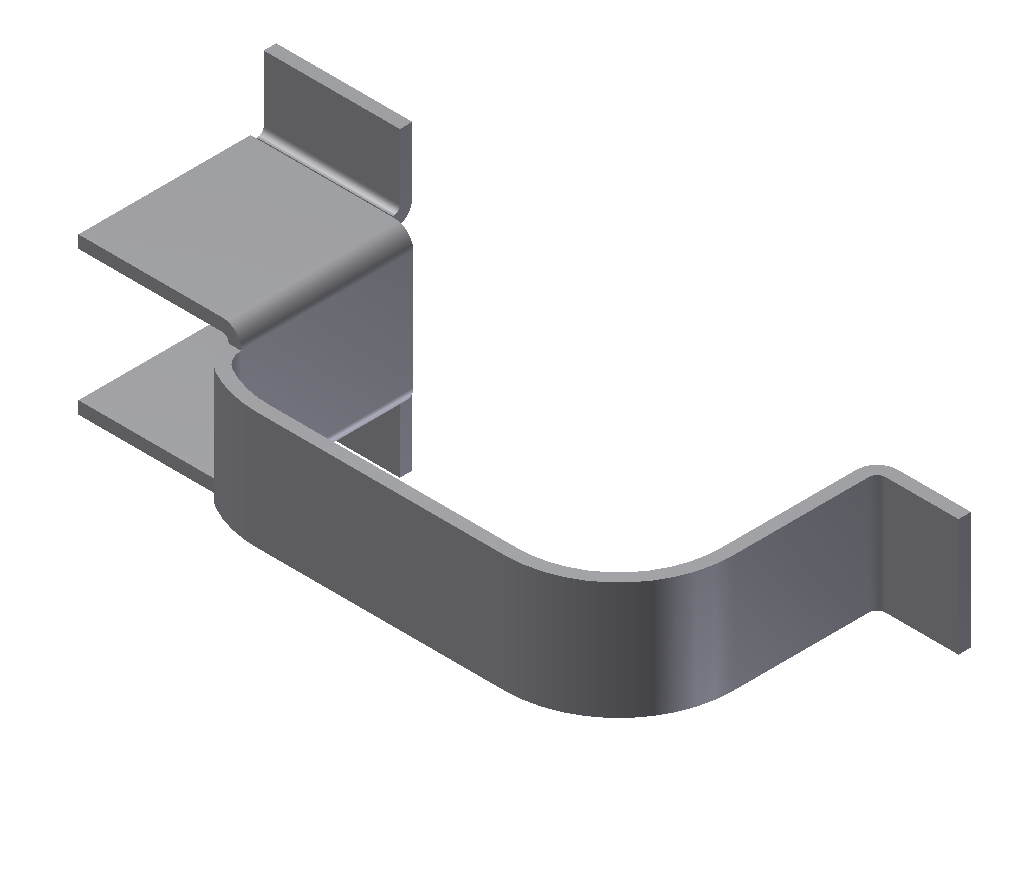
\includegraphics[width=0.98\linewidth]{images/ABELBracketOutputPart}} \\ \bottomrule
%
%\end{tabular}
%\captionof{figure}{Transformation of Sheet Metal features to  Generalized/Abstracted ($\mathcal{ABLE}$) forms}\label{fig:abel}
%\end{minipage}
%
%%%\bigskip

The output shows how the use of Spatial Grammar has made it possible to come up with a representation (as demonstrated by $\mathcal{ABLE}$) so that algorithms need not have to work with all sheet metal features but just a few generalized features.  Following section demonstrates how the generalized {\bf $\mathcal{ABLE}$} features compute the midsurface.

%%\section{Computing Midsurface of $\mathcal{ABLE}$ Model}
%%
%%Midsurface is a dimension reduction transformation from a solid to a surface. In the present research work the input CAD model with sheet metal features is converted to Loft-equivalent features in $\mathcal{ABLE}$ model. Thus computing midsurface reduces primarily to generating midsurface for Loft-equivalent{\bf $\mathcal{L}$} features, represented by 
%%
%%\loft{}{L}{3 }{0, curve, 0 | C_{0,1,2}}{ (sketch )^{<1-n>}}. This generalized Loft representation computes its corresponding midsurface as follows: 
%%
%%	\begin{enumerate}
%%	[noitemsep,topsep=2pt,parsep=2pt,partopsep=2pt]
%%	\item	{\bf $\mathcal{ABLE}$} Loft feature {\bf $\mathcal{L}$}'s parameters such as {\em sketches}, {\em guide curve} are extracted 
%%
%%\item Midcurve is computed from the {\em sketch} and Lofted with same feature parameters as that of  {\bf $\mathcal{L}$}. 
%%
%%This rule is expressed as \loft{}{L}{2}{0, guide, 0 | C_{0,1,2}}{midcurve^{1-n}} 
%%
%%
%%\begin{figure}[h]
%%\centering 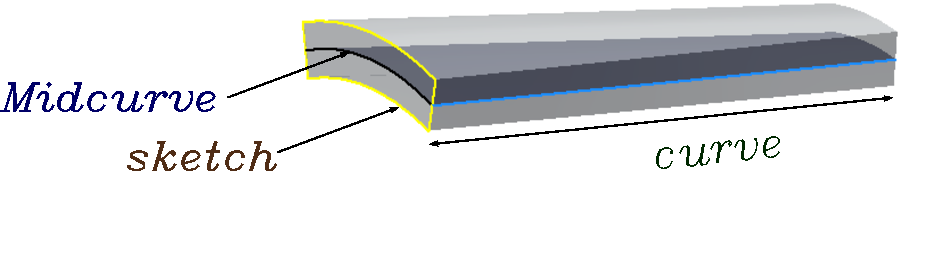
\includegraphics[scale=0.5]{images//MidsurfSmallProfile.pdf} 
%%%\caption{sketch is far smaller than guide}
%%\label{tbl:abstraction:midsurfsmallprofile}
%%\end{figure}
%%
%%Where, {\bf Midcurve} is a set of {\em curves} lying midway of a 2D {\em sketch}, is expressed as 	
%%
%%\generic{\Omega}{M}{}{C}{1}{} {sketch} 
%%\end{enumerate}
%%
%%\todo{Review Comment: This looks misfit here, Why here? [DELETED]} \deleted{Tree represented in the {\bf $\mathcal{ABLE}$} form becomes input to the Midsurface transformation operator. The feature tree's {\bf $\mathcal{ABLE}$} representation may other different types of operators, such as Transformation, Boolean, etc. For each, some action (or no-action) can be specified). For examples, as  {\bf $\mathcal{A}$} operators do not change topology and geometry type, Midsurface generated can follow just the same transformation as that of the parent shape. 
%%The {\bf $\mathcal{ABLE}$} then goes through cellular decomposition (Chapter \ref{ch:Midsurface}) where feature volumes are split. This converts feature interactions (Booleans) into cells. The cells retain the feature ({\bf $\mathcal{L}$}) ownership even after decomposition. Midsurface is generated for the  {\bf $\mathcal{L}$} portion that remains.
%%Advantage of the Spatial Grammar defined for Form Features is evident here in the sense one does not need to decide rules for all features, but just two - Loft and Boolean, and depending of different specifications they automatically become applicable to the rest of the forum features.}
%%
%%\todo{MY OPINION: NO NEED TO TALK ABOUT THICK THIN THERE, THATS NOT THE TOPIC, JUST TALK ABOUT MIDCURVE LOFTING CASE}

%%	\begin{enumerate}
%%	[noitemsep,topsep=2pt,parsep=2pt,partopsep=2pt]
%%	\item	{\bf $\mathcal{ABLE}$} Loft feature {\bf $\mathcal{L}$}'s parameters such as {\em sketches}, {\em guide curve} are extracted 
%%	\item Midsurface computation rules differ based on the ``thinness'' criteria, which in this case is based on the relative sizes of {\em sketch} and {\em guide}. As mentioned in Section \ref{sec:survey:intro}, though the criterion for ``thinness'' depends on the domain, $L/t > 2$ is considered for the present research.
%%	\item \added{Comparison is done betwwen $sketch_{size}$ and $guide_{size}$. Symbol $\ll$ suggests that length of the sketch has to be far less than length of the guide, for the {\bf $\mathcal{L}$} to get qualified for ``Thin Sketch'' (elaborated below) method of computing midsurface. $sketch$ being a 2D entity, its size (i.e. area) can not be compared directly with the size (i.e. length) of the $guide$. So, the present research takes summation of sketch curve lengths as the parameter denoting $sketch_{size}$, whereas $\ll$ is taken as factor of 2, meaning, $sketch_{size}$ has to at-least 2 times less that the $guide_{size}$.}
%%
%%\todo{Review comment: Be very careful for this. Sketch length is very significant term. What is the value of <<? who defines it? [ADDED SOME EXPLANATION]}
%%
%%\begin{itemize}[noitemsep,topsep=2pt,parsep=2pt,partopsep=2pt]
%%
%%
%%%\vspace{-1cm}
%%\item {\bf Thin Sketch}: If {\em sketch} is very small compared to {\em guide} ( $sketch_{size} \ll guide_{size}$), then {\em midcurve} is extracted from the {\em sketch} (as mentioned above) and {\em Lofted} with same feature parameters as that of  {\bf $\mathcal{L}$}. 
%%
%%This rule is expressed as \loft{}{L}{2}{0, guide, 0 | C_{0,1,2}}{midcurve^{1-n}} 
%%
%%
%%\begin{figure}[h]
%%\centering 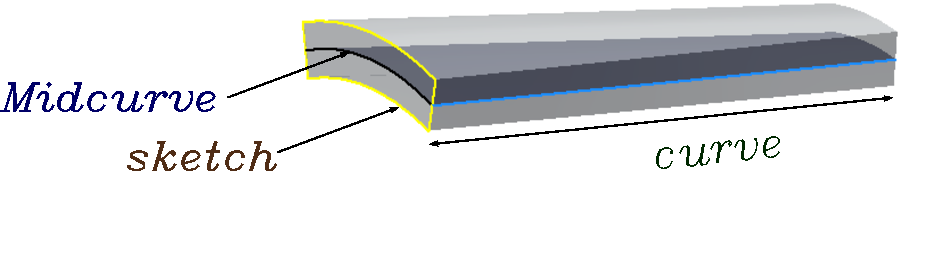
\includegraphics[scale=0.5]{images//MidsurfSmallProfile.pdf} 
%%%\caption{sketch is far smaller than guide}
%%\label{tbl:abstraction:midsurfsmallprofile}
%%\end{figure}
%%
%%Where, {\bf Midcurve} is a set of {\em curves} lying midway of a 2D {\em sketch}, is expressed as 	
%%
%%\generic{\Omega}{M}{}{C}{1}{} {sketch} 
%%
%%\item {\bf Thin Loft} :  If {\em sketch} is very big compared to {\em guide} ($sketch_{length} \gg guide_{length}$), then {\em midcurve} is not extracted  but the {\em sketch} itself is {\em Lofted} along half of the {\em guide}. This rule is expressed as
%%
%%\loft{}{L}{2}{0, guide/2, 0 | C_{0,1,2}}{sketch}.
%%%
%%%\begin{figure}[htbp]
%%%\centering 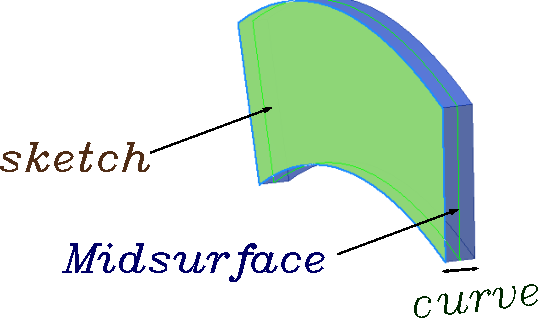
\includegraphics[scale=0.40]{images//MidsurfSmallCurve.pdf}
%%%\caption{sketch is far bigger than guide}
%%%\label{figure_MidsurfSmallCurve}
%%%\end{figure}
%%
%%\item {\bf Thick Sketch}:   If {\em sketch} is comparable in size to {\em guide}  ($sketch_{length} \approx guide_{length}$), then it is a thick shape and Midsurface is not generated.
%%\end{itemize}
%%\end{enumerate}

%
%
%For {\bf $\mathcal{B}$} operators rules are devised depending on where the target and tools have Midsurface extracted already.
%%\vspace{-0.2cm}
%
%\begin{itemize}[noitemsep,topsep=2pt,parsep=2pt,partopsep=2pt]
%
%\item {\bf Union} : If the {\em target} and the {\em tool bodies} have midsurfaces, extend the midsurfaces to join at the common intersections.
%
%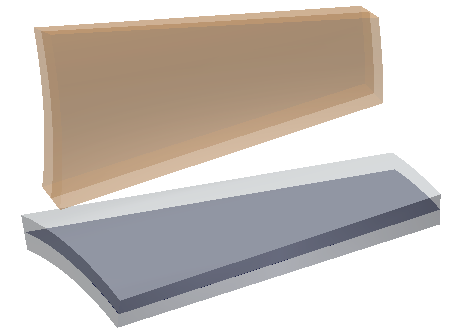
\includegraphics[scale=0.45]{images//Midsurf_unite.png} 
%
%\item {\bf Difference-Thin} : If {\em target} is thin then irrespective of {\em tool bodies'} thickness, are subtracted.
%
%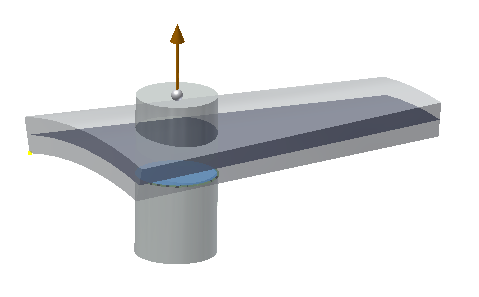
\includegraphics[scale=0.45]{images//Midsurf_diffthin.png}
%
%\item {\bf Difference-Thick} : If {\em target} and {\em tool bodies} are thick and are in {\em Shell} like situation, {\em midcurves} of combined {\em sketches} are calculated and {\em Lofted}  
%
%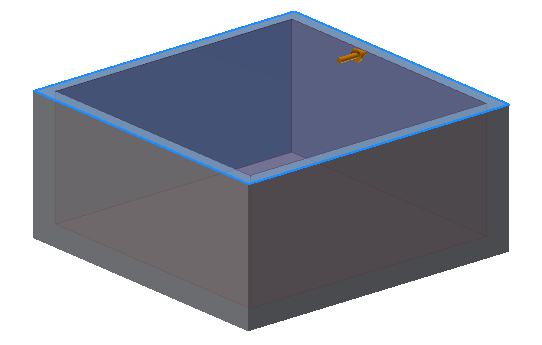
\includegraphics[scale=0.32]{images//Midsurf_diffthick.png}
%\end{itemize}
%
%As for implementation, a {\em feature based} CAD model is taken as an input. Using direct access or via Application Programming Interface (APIs), {\em feature tree} is queried. A {\em feature tree} is a chronological list of {\em features} stored as part gets built. Each feature is traversed one by one, and wherever applicable, a corresponding Midsurface is extracted. For {\em features} like {\em Extrude} which may have internal-{\em boolean}, two separate {\em features} are modeled, one for {\em tool body} creation by {\em Extrude} and the second one as {\em Boolean}.

%\begin{table}[htbp]
%\begin{tabular}{  p{0.3\textwidth} p{0.1\textwidth} }
%
%{\bf Union} : If {\em target} and {\em tool bodies} are thin, extend midsurfaces from both and join at common intersection &	
%
%\raisebox{-0.6in}{\includegraphics[scale=0.25]{images//Midsurf_unite.png} } \\
%
%{\bf Difference-Thin} : If {\em target} is thin having Midsurface, then irrespective whether {\em tool bodies} are thick or thin, they cut the Midsurface of {\em target} & 
%
%\raisebox{-0.6in}{\includegraphics[scale=0.25]{images//Midsurf_diffthin.png} } \\
%
%{\bf Difference-Thick} : If {\em target} and {\em tool bodies} are thick and are in shell like situation, {\em midcurves} of combined {\em sketches} is calculated and {\em Lofted}  & 
%
%\raisebox{-0.6in}{\includegraphics[scale=0.18]{images//Midsurf_diffthick.png} } \\

%\end{tabular}
%\caption{Midsurface of Boolean Operators}
%\label{table_BoolMidsurf}
%\end{table}


%\subsection{Generic Programming for Midsurface Algorithm}
%Form Feature operators developed in $\mathcal{ABLE}$ can be directly mapped to hierarchy of {\em Trait} classes (Figure ~\ref{figure_Traits}).
%
%\begin{figure}[h]
%\begin{center}
%
%%\includegraphics[scale=0.45]{images//Traits_hierarchy.pdf}
%
%\tikzset{edge from parent/.style= {draw, edge from parent path={(\tikzparentnode.south) -- +(0,-8pt) -| (\tikzchildnode)}}, blank/.style={draw=none}}
%
%\resizebox{\linewidth}{!}{%
%\begin{tikzpicture}
%\node{\Tree 
%[.{Regulator\_Traits\{\}} 
%    	[.{Affine\_Traits\{\}} 
%        	[{} {Translate\_Traits} {}	] 
%	]
%    	[.{Boolean\_Traits\{\}}  
%		[{} {Union\_Traits} {}	]
%	]
%    	[.{Loft\_Traits\{\}}  
%		[{} {Sweep\_Traits} {Extrude\_Traits}{}	]
%	]
%]};
%\end{tikzpicture}
%}
%\end{center}
%\caption{Traits Hierarchy}
%\label{figure_Traits}
%\end{figure}
%
%\begin{algorithm}
%	\caption{Midsurface Generation}
%	\label{alg1}
%	\begin{algorithmic}
%		\REQUIRE Feature Tree Iterator
%		\ENSURE All the features have corresponding Traits available
%
%		\WHILE{Feature Iterator continues to advance}
%			\STATE Get current Feature Trait.
%			\IF {Trait is of type Loft Trait}           
%			\STATE  Midcurves are generated from {\em sketches(s)} and lofted along with {\em guide curve}.
%			\ENDIF
%
%			\IF {Trait is of type Boolean Trait}           
%			\STATE  boolean process mentioned before is followed to connect/cut the Midsurface.
%			\ENDIF
%
%			\IF {Trait is of type Affine Transformation Trait}           
%			\STATE  simply same transformation is applied to the Midsurface also.
%			\ENDIF
%
%		\ENDWHILE
%		\STATE  Each feature, if applicable, contributes to building connected Midsurface model.
%	\end{algorithmic}
%\end{algorithm}
%
%In a typical process (Algorithm~\ref{alg1}), {\em feature iterator} is used to traverse {\em feature tree} and  the corresponding {\em Trait} representation is extracted from each feature. Midsurface Algorithms specializations based on each {\em Trait} type get automatically invoked. The process continues till the end of the {\em feature tree}.
%
%
%Advantages of this systems is that any feature tree who can generate the  $\mathcal{ABLE}$ {\em Trait} system can utilize the Midsurface algorithm, making it portable across various feature schema.
%%
%%\section{Feature Taxonomy}
%%
%%%\includegraphics[scale=0.35]{images/ThinWallFeaturesTaxonomy.png}
%%
%%\resizebox{\linewidth}{!}{% for scaling the whole tree
%%\begin{tikzpicture}
%%\tikzset{grow'=down}
%%%\tikzset{every tree node/.style={font=\small}} %No effect
%%\tikzset{every tree node/.style={align=center}}
%%\tikzset{sibling distance=6pt}
%%\tikzset{level distance=60pt}
%%\tikzset{edge from parent/.style=
%%{draw, edge from parent path={(\tikzparentnode.south) -- +(0,-8pt) -| (\tikzchildnode)}}, blank/.style={draw=none}}
%%\node{\Tree [.{Thin Wall Part Features}
%%		[.{non Profile based} 
%%			Shell
%%			[.Boolean Additive Subtractive
%%			]
%%			{Fillet\\ Chamfer}
%%			{Spot\\ Weld\\ Rivette}
%%		]
%%		[.{Profile based} 
%%			[.{Thin Profile Long Directrix}
%%				[.{Curved Directrix\\ w or w/out draft} Flange ThinSweep {Hem\\ Teardrop} {Drawing\\ Stamping\\ Coining} ]
%%				[.{Circular Directrix\\ w or w/out draft} Bend ThinRevolve ] 
%%				[.{Linear Directrix\\ w or w/out draft} ThinExtrude ] 
%%			] 
%%			[.{Thick Profile Short -Linear Directrix}
%%				[.Subtractive {Cutout\\ Hole} ]
%%				[.Additive ThickExtrude {Face\\ Wall} ] 
%%			] 
%%		]
%%	]
%%};
%%
%%\end{tikzpicture}
%%} %resizebox

\section{Significance of $\mathcal{ABLE}$ Paradigm}
This chapter elaborates the proposed $\mathcal{ABLE}$ representation implemented in \mysystemname~system. Significance of using $\mathcal{ABLE}$ based feature-definition is enumerated below:
	\begin{enumerate} [noitemsep,topsep=2pt,parsep=2pt,partopsep=2pt]
	\item Spatial Grammar, which has been largely used in exploratory, generative and architectural applications, has been used in the present research to represented mechanical engineering CAD features in a generic way so that they can be applicable in various CAD systems. 
%	\item Midsurface transformation has been defined on the generalized feature definitions, demonstrating generic and concise way of devising feature-based algorithms.
%	\item  $\mathcal{ABLE}$ is independent of different CAD systems. Features from these systems can be transformed into $\mathcal{ABLE}$ features and thus same midsurface computation algorithm can be used without modifications.
	\item Features which are similar in nature can be put in a single category in $\mathcal{ABLE}$. All sketch based features, such as, Extrude, Revolve, Sweep, Loft can be under $SketchFeature$ category and then individual types can be the `subtype' field.
	\item In case of feature based modeling, although variation in parameters is possible, changing the shape dramatically is not possible (to an extent it is possible with Replace Face kind of features), but Shape Grammars are very generic and can generate wide range of shapes. Feature-definition-constraint rules, should be imposed to restrict allowable changes only.
	\end{enumerate}

Following section elaborates generation of {\bf $\mathcal{ABLE}$} model for a practical part model.

